
\documentclass[10pt,a4paper]{article}
\usepackage{fontspec}
\usepackage{polyglossia}
\setdefaultlanguage{russian}
\setotherlanguage{english}
\setmainfont{Segoe UI}
\setsansfont{Segoe UI}
\setmonofont{Consolas}[Scale=0.92]

\usepackage[a4paper,top=2.0cm,bottom=2.0cm,left=1.9cm,right=1.9cm,headheight=14pt]{geometry}
\usepackage[table]{xcolor}
\definecolor{vk}{HTML}{0077FF}
\definecolor{navy}{HTML}{0B2A5B}
\definecolor{blue}{HTML}{0B3D91}
\definecolor{dark}{HTML}{1F2733}
\definecolor{grey}{HTML}{667085}
\definecolor{light}{HTML}{E6ECF5}
\definecolor{soft}{HTML}{F4F7FB}
\definecolor{zebra}{HTML}{F4F7FB}

\usepackage{longtable}
\usepackage{array}
\usepackage{booktabs}
\usepackage{enumitem}
\usepackage{graphicx}
\usepackage{caption}
\usepackage{amssymb}
\usepackage{ragged2e}
\usepackage{titlesec}
\usepackage{fancyhdr}
\usepackage{lastpage}
\usepackage[hidelinks]{hyperref}

\hypersetup{
  pdftitle={Социальная коммерция ВКонтакте: результаты исследования},
  pdfauthor={Команда проекта},
  pdfsubject={VK Case Championship 2026, handover-документ},
  pdfkeywords={ВКонтакте, социальная коммерция, Маркет, e-commerce}
}

\linespread{1.12}
\setlength{\parindent}{0pt}
\setlength{\parskip}{5pt plus 1pt}
\setlength{\emergencystretch}{3em}
\sloppy

\captionsetup{font={small,color=grey},justification=centering,skip=5pt}
\setlength{\LTpre}{6pt}
\setlength{\LTpost}{10pt}

\titleformat{\section}
  {\Large\bfseries\color{navy}}{\thesection}{0.55em}{}
  [\vspace{-2pt}{\color{light}\titlerule[1.1pt]}]
\titlespacing*{\section}{0pt}{6pt}{12pt}
\titleformat{\subsection}
  {\large\bfseries\color{blue}}{\thesubsection}{0.5em}{}
\titlespacing*{\subsection}{0pt}{14pt}{6pt}
\titleformat{\subsubsection}
  {\normalsize\bfseries\color{dark}}{\thesubsubsection}{0.5em}{}
\titlespacing*{\subsubsection}{0pt}{10pt}{4pt}

\pagestyle{fancy}
\fancyhf{}
\fancyhead[L]{\footnotesize\color{grey}VK Case Championship 2026\ \textbullet\ handover}
\fancyhead[R]{\footnotesize\color{grey}\nouppercase{\leftmark}}
\fancyfoot[C]{\footnotesize\color{grey}стр. \thepage\ из \pageref{LastPage}}
\renewcommand{\headrulewidth}{0.4pt}
\renewcommand{\headrule}{\hbox to\headwidth{\color{light}\leaders\hrule height \headrulewidth\hfill}}
\renewcommand{\footrulewidth}{0pt}

\begin{document}


\begin{titlepage}
\thispagestyle{empty}
\noindent\colorbox{vk}{\parbox{\dimexpr\linewidth-2\fboxsep}{
\color{white}\small\bfseries VK CASE CHAMPIONSHIP 2026\ \ \textbullet\ \ ОТБОРОЧНЫЙ ЭТАП\ \ \textbullet\ \ КЕЙС «СОЦИАЛЬНАЯ КОММЕРЦИЯ»}}\par
\vspace*{56pt}
{\raggedright\fontsize{26}{31}\selectfont\bfseries\color{navy}Социальная коммерция ВКонтакте\par}
\vspace{2pt}
{\raggedright\fontsize{21}{26}\selectfont\bfseries\color{blue}результаты исследования\par}
\vspace{16pt}
{\Large\color{grey}Handover-документ для команды\par}
\vspace{30pt}
{\color{light}\rule{\linewidth}{1.2pt}}\par
\vspace{12pt}
{\small\color{dark}\raggedright VK Case Championship 2026 · отборочный этап · кейс «Развитие элементов социальной коммерции для бизнес-сообществ во ВКонтакте»\par}
{\small\color{dark}\raggedright Дата: 15 ноября 2026 · Версия 1.0 · Период данных: сентябрь 2026 · Выборка: 9 754 бизнес-сообщества\par}
\vspace{18pt}
\noindent\colorbox{soft}{\parbox{\dimexpr\linewidth-2\fboxsep}{
\raggedright\color{navy}\textbf{Как пользоваться документом.} Это не презентация и не финальный ответ, а рабочая база: здесь собраны проверенные числа, интерпретации, границы применимости и готовые формулировки для слайдов. Всё, что можно пересчитать, лежит в \texttt{outputs/} и воспроизводится командой \texttt{python run\_all.py}. Если меняете число — меняйте его в ноутбуке, а не в тексте.
}}
\vfill
{\footnotesize\color{grey}Материалы для команды: числа, логика, границы выводов и заготовки слайдов.\ Все расчёты воспроизводятся командой \texttt{python run\_all.py}.\par}
\end{titlepage}

\setcounter{page}{2}

\clearpage

{\small

\tableofcontents

}

\clearpage

\section{Три минуты: главное}

\begin{enumerate}[leftmargin=1.35em,itemsep=2pt,topsep=3pt,parsep=0pt]
\item \textbf{Проблема не в спросе, а в замыкании сделки.} У ВКонтакте 90,8 млн DAU и более миллиона бизнес-сообществ, но только \textbf{3,1\%} сообществ выборки имеют хотя бы один заказ через чекаут. Из 5 737 сообществ с подключённым чекаутом продают \textbf{284}, то есть \textbf{4,95\%}; \textbf{94,8\%} «спят».
\item \textbf{Узкое место — шаг «открытие карточки → нажатие кнопки».} У Маркета ВКонтакте он даёт \textbf{3,08\%} против \textbf{42,16\%} у Партнёра 1. На этот шаг приходится \textbf{106\%} логарифмического разрыва в заказах; состав категорий объясняет \textbf{−14\%}, а механика внутри категорий — \textbf{+114\%}.
\item \textbf{Инструменты не работают по отдельности.} Ассортимент — сильнейший наблюдаемый предиктор первой продажи (OR≈1,52 на e× каталога, топ-1 важность в ML). Доставка наивно даёт ×3,2, но после PSM — лишь \textbf{+2,8…3,5 п.п.}, и во всех 8 спецификациях доверительный интервал включает ноль. Это не «доставка не нужна», это «доставка без каталога, трафика и исполнения не создаёт продажу».
\item \textbf{Товарный контент — канал охвата, а не конверсии.} Товарные публикации получают в \textbf{1,9 раза} больше просмотров на публикацию, но их ER в \textbf{1,8 раза} ниже, а CTR в карточку — \textbf{0,29\%}. Публикуют товарный контент только \textbf{3,1\%} сообществ. Потенциал — в формате и CTA, а не в количестве постов.
\item \textbf{Реклама не доказала связь с продажей.} 542 сообщества платят за рекламу; у \textbf{501 (92,4\%)} нет измеримого заказа, на них приходится \textbf{87,6\%} бюджета. Связь трат с вероятностью первой продажи статистически незначима (OR≈1,02, p=0,31). Модель «продавать трафик» упирается в потолок доверия.
\item \textbf{Стратегический ответ — не строить второй маркетплейс, а стать слоем сделки.} Маркет ВКонтакте — это \textbf{0,14\% GMV} и \textbf{0,06\% заказов} рынка e-com РФ, его DAU — \textbf{0,14\%} от DAU ВКонтакте. Зато 27,3 млн человек в месяц открывают карточки, а 28,6 млн запросов в товарном поиске ждут интента. Нужно превратить Маркет из «места» в \textbf{инфраструктуру: каталог + карточка-сделка + чекаут + доставка/оплата + поиск + профиль покупателя}.
\item \textbf{Целевой сегмент — S4 «спящий магазин»: 2 922 сообщества, 30\% выборки, 5,3\% продающих.} Это ядро активации: у них уже есть каталог и чекаут, но нет доставки/оплаты. S2 (2 096) — быстрый прирост через импорт каталога, S3 (320) — quick win, S5/S6 (719) — рост объёма и монетизации. S0/S1 (3 697) — вне фокуса кейса.
\item \textbf{Базовая модель:} 1,70 млн заказов/мес и 5,62 млрд ₽ GMV/мес; новая выручка от комиссии и подписки — \textbf{143 млн ₽/мес} (1,72 млрд ₽/год). Консервативный сценарий — 774 тыс. заказов и 21 млн ₽/мес; агрессивный — 4,35 млн заказов и 633 млн ₽/мес. Это не прогноз, а модель «что если» с явными допущениями.
\item \textbf{Главный риск — переоценить эффект.} Наблюдательные данные, self-selection, один месяц, 98,8\% заказов не оплачены внутри VK. Все обещания должны идти через A/B и сопровождаться доверительными интервалами. В отчёте есть отдельный список «что нельзя утверждать».
\end{enumerate}

\clearpage

\section{Контекст кейса и требования из PDF}

\subsection{Что просит кейс}

Кейс — про \textbf{социальную коммерцию для бизнес-сообществ}, а не про авторов и не про рекламный кабинет. Ключевая цель сформулирована на слайде постановки задачи:\par

\begin{quote}
\noindent\colorbox{soft}{\parbox{\dimexpr\linewidth-2\fboxsep}{
\raggedright \textbf{Увеличить число бизнесов, продающих через ВКонтакте. Ориентиры — число бизнесов, подключивших инструменты продаж, и число заказов, оформленных внутри ВКонтакте.}
}}
\end{quote}
\vspace{2pt}

Из этого следуют два измерения успеха, которые нельзя путать:\par

\begingroup
\small
\setlength{\tabcolsep}{3pt}
\renewcommand{\arraystretch}{1.12}
\rowcolors{1}{white}{zebra}
\begin{longtable}{@{}>{\raggedright\arraybackslash}p{0.1288\linewidth}>{\raggedright\arraybackslash}p{0.4233\linewidth}>{\raggedright\arraybackslash}p{0.4233\linewidth}@{}}
\rowcolor{blue}
\textcolor{white}{\textbf{Измерение}} & \textcolor{white}{\textbf{Метрика кейса}} & \textcolor{white}{\textbf{Где она живёт в модели}} \\
\endfirsthead
\rowcolor{blue}
\textcolor{white}{\textbf{Измерение}} & \textcolor{white}{\textbf{Метрика кейса}} & \textcolor{white}{\textbf{Где она живёт в модели}} \\
\endhead
\hline
Ширина воронки & число бизнесов, подключивших инструменты продаж & доля сообществ с каталогом, чекаутом, доставкой, оплатой \\
Глубина сделки & число заказов, оформленных внутри ВКонтакте & заказы/мес, GMV/мес, оплаченные заказы \\
\hline
\end{longtable}
\endgroup
\vspace{4pt}

\textbf{Практический вывод:} сначала растёт «ширина» (подключение), потом «глубина» (заказы). Нельзя отчитываться только подключениями: 94,8\% подключивших чекаут не продают.\par

\subsection{Пять задач кейса}

\begingroup
\small
\setlength{\tabcolsep}{3pt}
\renewcommand{\arraystretch}{1.12}
\rowcolors{1}{white}{zebra}
\begin{longtable}{@{}>{\raggedright\arraybackslash}p{0.0347\linewidth}>{\raggedright\arraybackslash}p{0.3991\linewidth}>{\raggedright\arraybackslash}p{0.3991\linewidth}>{\raggedright\arraybackslash}p{0.1301\linewidth}@{}}
\rowcolor{blue}
\textcolor{white}{\textbf{№}} & \textcolor{white}{\textbf{Задача}} & \textcolor{white}{\textbf{Что должно быть в ответе}} & \textcolor{white}{\textbf{Где в отчёте}} \\
\endfirsthead
\rowcolor{blue}
\textcolor{white}{\textbf{№}} & \textcolor{white}{\textbf{Задача}} & \textcolor{white}{\textbf{Что должно быть в ответе}} & \textcolor{white}{\textbf{Где в отчёте}} \\
\endhead
\hline
1 & Определить место ВКонтакте для бизнеса среди маркетплейсов, классифайдов и других каналов & анализ рынка, российские и международные практики, позиционирование & раздел 5.1, 4.1 \\
2 & Выбрать целевые бизнесы: что им нужно, чего хотят, с какими трудностями сталкиваются; что мешает расти; как помочь & сегменты, барьеры, приоритеты & раздел 4.2, 5.2 \\
3 & Сформулировать уникальное предложение и инструменты продвижения, продаж, работы с клиентами; эффект для бизнеса и VK & ценностное предложение, 5 рычагов, таблица двухсторонних эффектов & раздел 6, 5.3 \\
4 & Проанализировать данные и открытые источники, определить роль Маркета ВКонтакте & альтернативы A/B/C, выбранная роль, метрики & раздел 4.1, 5.4 \\
5 & Спроектировать и обосновать целевой путь бизнеса от первого контакта до продажи, с развилками и инструментами на каждом этапе & карта пути, развилки по сегментам, метрики этапов & раздел 7, 5.5 \\
\hline
\end{longtable}
\endgroup
\vspace{4pt}

\subsection{Требования к сдаче}

\begingroup
\small
\setlength{\tabcolsep}{3pt}
\renewcommand{\arraystretch}{1.12}
\rowcolors{1}{white}{zebra}
\begin{longtable}{@{}>{\raggedright\arraybackslash}p{0.1764\linewidth}>{\raggedright\arraybackslash}p{0.8113\linewidth}@{}}
\rowcolor{blue}
\textcolor{white}{\textbf{Требование}} & \textcolor{white}{\textbf{Деталь}} \\
\endfirsthead
\rowcolor{blue}
\textcolor{white}{\textbf{Требование}} & \textcolor{white}{\textbf{Деталь}} \\
\endhead
\hline
Формат & презентация PDF, \textbf{8 слайдов} \\
Приложения & без ограничений по количеству \\
Имя файла & \texttt{название команды\_strategy\_msk/spb} \\
Дедлайн & \textbf{22 ноября, 09:00}; одна заявка от команды; доступ к файлам не закрывать до конца чемпионата \\
Структура & титул → команда и город → Executive Summary → проблематика → альтернативы → выбранная концепция → обоснование → выводы и рекомендации \\
Критерии & глубина, широта, структура и логика, соответствие задаче, анализ датасета, качество презентации \\
ИИ & использование раскрыть: какие инструменты, для каких задач, чем помогли; результаты проверить \\
\hline
\end{longtable}
\endgroup
\vspace{4pt}

\textbf{Важно:} PDF прямо говорит, что кейс не предполагает единственного верного решения, а часть данных могла быть намеренно искажена или упрощена. Поэтому в презентации нужно не «угадать ответ», а показать \textbf{логику, расчёты, альтернативы и границы}. Это же требование к глубине и широте анализа.\par

\subsection{Критерии оценки — как их закрывать}

\begingroup
\small
\setlength{\tabcolsep}{3pt}
\renewcommand{\arraystretch}{1.12}
\rowcolors{1}{white}{zebra}
\begin{longtable}{@{}>{\raggedright\arraybackslash}p{0.2206\linewidth}>{\raggedright\arraybackslash}p{0.5341\linewidth}>{\raggedright\arraybackslash}p{0.2206\linewidth}@{}}
\rowcolor{blue}
\textcolor{white}{\textbf{Критерий}} & \textcolor{white}{\textbf{Что делать в deck}} & \textcolor{white}{\textbf{Артефакт}} \\
\endfirsthead
\rowcolor{blue}
\textcolor{white}{\textbf{Критерий}} & \textcolor{white}{\textbf{Что делать в deck}} & \textcolor{white}{\textbf{Артефакт}} \\
\endhead
\hline
Глубина & показать механику: воронка, декомпозиция, PSM, чувствительность & рис. 3–6, 8–10 \\
Широта & рынок, сегменты, инструменты, финансы, риски, план & разделы 4–9 \\
Структура и логика & единая линия: проблема → альтернативы → концепция → обоснование → выводы & раздел 10 \\
Соответствие задаче & явно ответить на 5 вопросов, не уходить в услуги и авторов & раздел 5 \\
Анализ датасета & числа из данных, не «экспертные ощущения»; указать ограничения & разделы 3–4 \\
Качество & деловой стиль, аккуратные графики, без опечаток & приложение, figures \\
\hline
\end{longtable}
\endgroup
\vspace{4pt}

\clearpage

\section{Данные, метод и границы выводов}

\subsection{Что в датасете}

Датасет — 7 листов Excel за сентябрь 2026:\par

\begingroup
\small
\setlength{\tabcolsep}{3pt}
\renewcommand{\arraystretch}{1.12}
\rowcolors{1}{white}{zebra}
\begin{longtable}{@{}>{\raggedright\arraybackslash}p{0.1751\linewidth}>{\raggedright\arraybackslash}p{0.2126\linewidth}>{\raggedright\arraybackslash}p{0.2877\linewidth}>{\raggedright\arraybackslash}p{0.2877\linewidth}@{}}
\rowcolor{blue}
\textcolor{white}{\textbf{Лист}} & \textcolor{white}{\textbf{Гранулярность}} & \textcolor{white}{\textbf{Что даёт}} & \textcolor{white}{\textbf{Ограничение}} \\
\endfirsthead
\rowcolor{blue}
\textcolor{white}{\textbf{Лист}} & \textcolor{white}{\textbf{Гранулярность}} & \textcolor{white}{\textbf{Что даёт}} & \textcolor{white}{\textbf{Ограничение}} \\
\endhead
\hline
Бизнесы & сообщество × 30 дней, 9 754 строки & сегменты, инструменты, контент, заказы через чекаут, реклама & нет продаж мимо чекаута (сообщения, внешний сайт) \\
Маркет ВКонтакте — итоги & сегмент × 30 дней, 26 строк & воронка, GMV, покупатели, DAU/MAU & у Партнёра нет «оплаченных заказов» \\
Маркет ВКонтакте — по дням & день × сегмент, 30 дней & динамика, тренды, день недели & уникальных покупателей нельзя суммировать по дням \\
Маркет ВКонтакте — источники & источник × сегмент & структура открытий карточки & нет заказов в разрезе источника \\
Маркет ВКонтакте — категории & категория × сегмент, 18 категорий & конверсия и ассортиментный разрыв & суммы заказов расходятся с итогами на 5–7\% \\
Покупатели & пол × возраст × сегмент & профиль покупателя, заказы на покупателя & группы <100 скрыты \\
Покупатели по регионам & регион × сегмент, 89 регионов & гео-концентрация & нет населения регионов, группы <100 скрыты \\
\hline
\end{longtable}
\endgroup
\vspace{4pt}

\subsection{Выборка — не вся платформа}

Это первое, что нужно проговорить на защите, иначе любое «умножение на миллион» будет ошибкой.\par

\begingroup
\small
\setlength{\tabcolsep}{3pt}
\renewcommand{\arraystretch}{1.12}
\rowcolors{1}{white}{zebra}
\begin{longtable}{@{}>{\raggedright\arraybackslash}p{0.4433\linewidth}>{\raggedright\arraybackslash}p{0.1376\linewidth}>{\raggedright\arraybackslash}p{0.1987\linewidth}>{\raggedright\arraybackslash}p{0.1834\linewidth}@{}}
\rowcolor{blue}
\textcolor{white}{\textbf{Показатель}} & \textcolor{white}{\textbf{Выборка}} & \textcolor{white}{\textbf{Платформа}} & \textcolor{white}{\textbf{Доля выборки}} \\
\endfirsthead
\rowcolor{blue}
\textcolor{white}{\textbf{Показатель}} & \textcolor{white}{\textbf{Выборка}} & \textcolor{white}{\textbf{Платформа}} & \textcolor{white}{\textbf{Доля выборки}} \\
\endhead
\hline
Заказы оформленные & 3 478 & 413 740 & 0,84\% \\
Заказы оплаченные & 3 478 & 4 903 & \textbf{70,9\%} \\
GMV, ₽ & 9 973 027 & 1 564 546 740 & \textbf{0,64\%} \\
Открытия карточки из контента & 53 068 & 86 321 893 & 0,06\% \\
\hline
\end{longtable}
\endgroup
\vspace{4pt}

Выборка \textbf{перепредставлена оплаченными заказами} (70,9\% всех оплаченных заказов платформы) и \textbf{недопредставлена GMV} (0,64\%). Поэтому:\par

\begin{itemize}[leftmargin=1.35em,itemsep=2pt,topsep=3pt,parsep=0pt]
\item \textbf{нельзя} экстраполировать абсолютные заказы и GMV выборки на платформу;
\item \textbf{можно} переносить структуру, доли, относительные эффекты и направления;
\item для платформенных сценариев считаем от платформенных метрик (413,7 тыс. заказов, 1,56 млрд ₽), а не от выборки.
\end{itemize}

\subsection{Аномалии и как мы с ними обращались}

\begingroup
\small
\setlength{\tabcolsep}{3pt}
\renewcommand{\arraystretch}{1.12}
\rowcolors{1}{white}{zebra}
\begin{longtable}{@{}>{\raggedright\arraybackslash}p{0.3187\linewidth}>{\raggedright\arraybackslash}p{0.0485\linewidth}>{\raggedright\arraybackslash}p{0.2771\linewidth}>{\raggedright\arraybackslash}p{0.3187\linewidth}@{}}
\rowcolor{blue}
\textcolor{white}{\textbf{Аномалия}} & \textcolor{white}{\textbf{Масштаб}} & \textcolor{white}{\textbf{Почему проблема}} & \textcolor{white}{\textbf{Решение}} \\
\endfirsthead
\rowcolor{blue}
\textcolor{white}{\textbf{Аномалия}} & \textcolor{white}{\textbf{Масштаб}} & \textcolor{white}{\textbf{Почему проблема}} & \textcolor{white}{\textbf{Решение}} \\
\endhead
\hline
Чекаут подключён, каталог пуст & 2 096 & технически чекаут без товаров невозможен & выделен в S2, не считается «готовым к продажам» \\
Просмотры товарного контента без публикаций с товаром & 1 013 & разная атрибуция окон & парные тесты только там, где есть и публикации, и просмотры \\
Открытия карточки > просмотров товарного контента & 40 & нарушение вложенности воронки & исключены из CTR карточки \\
Заказы > 0, GMV = 0 & 7 & незаполненные суммы & AOV считаем на агрегате \\
Доставка или оплата без чекаута & 168 & нарушение логики стека & строгая вложенность в воронке \\
«Средний чек» ≠ GMV/заказы & 291 & медианное отношение ≈1,18 & везде расчётный AOV = GMV/заказы \\
\hline
\end{longtable}
\endgroup
\vspace{4pt}

Дополнительно: суммы заказов по категориям расходятся с итогами на \textbf{+5,2\%} (Маркет) и \textbf{−7,5\%} (Партнёр); открытия «из постов и клипов» расходятся с источниками «Лента + Клипы» на \textbf{−26\%} из-за разной атрибуции. Поэтому в категорийном анализе смотрим на структуру и отношения, а не на абсолютные суммы.\par

\subsection{Методы}

\begingroup
\small
\setlength{\tabcolsep}{3pt}
\renewcommand{\arraystretch}{1.12}
\rowcolors{1}{white}{zebra}
\begin{longtable}{@{}>{\raggedright\arraybackslash}p{0.3116\linewidth}>{\raggedright\arraybackslash}p{0.1062\linewidth}>{\raggedright\arraybackslash}p{0.3257\linewidth}>{\raggedright\arraybackslash}p{0.2195\linewidth}@{}}
\rowcolor{blue}
\textcolor{white}{\textbf{Метод}} & \textcolor{white}{\textbf{Где}} & \textcolor{white}{\textbf{Зачем}} & \textcolor{white}{\textbf{Что не даёт}} \\
\endfirsthead
\rowcolor{blue}
\textcolor{white}{\textbf{Метод}} & \textcolor{white}{\textbf{Где}} & \textcolor{white}{\textbf{Зачем}} & \textcolor{white}{\textbf{Что не даёт}} \\
\endhead
\hline
Сегментация по стеку инструментов & ноутбук 01 & выделить S0–S6 и целевые группы & не является causal-дизайном \\
Воронка и декомпозиция шагов & ноутбук 03 & найти узкое место & не объясняет, почему шаг плохой \\
Логит + ML & ноутбук 02 & какие признаки связаны с первой продажей & ассоциация, не эффект \\
PSM & ноутбуки 02, 05 & скорректировать self-selection по наблюдаемым признакам & не убирает ненаблюдаемый отбор \\
Разложение «состав vs механика» & ноутбук 05 & отделить микс категорий от конверсии внутри категорий & 17 категорий, суммы не сходятся \\
Тренды с фиксированными эффектами дня недели & ноутбук 05 & убрать календарный артефакт & 30 наблюдений, нет сезонности \\
Сценарная модель & ноутбук 04 & оценить порядок эффекта и чувствительность & не прогноз; допущения явные \\
\hline
\end{longtable}
\endgroup
\vspace{4pt}

\subsection{Статус доказательности}

Договоримся о языке, чтобы не спорить на защите:\par

\begingroup
\small
\setlength{\tabcolsep}{3pt}
\renewcommand{\arraystretch}{1.12}
\rowcolors{1}{white}{zebra}
\begin{longtable}{@{}>{\raggedright\arraybackslash}p{0.1121\linewidth}>{\raggedright\arraybackslash}p{0.3475\linewidth}>{\raggedright\arraybackslash}p{0.5157\linewidth}@{}}
\rowcolor{blue}
\textcolor{white}{\textbf{Статус}} & \textcolor{white}{\textbf{Что это}} & \textcolor{white}{\textbf{Пример}} \\
\endfirsthead
\rowcolor{blue}
\textcolor{white}{\textbf{Статус}} & \textcolor{white}{\textbf{Что это}} & \textcolor{white}{\textbf{Пример}} \\
\endhead
\hline
\textbf{Факт} & прямо измерено в данных & 3,08\% открытие→кнопка у Маркета \\
\textbf{Ассоциация} & устойчивая связь после контроля & доставка связана с +3 п.п. активации после PSM \\
\textbf{Гипотеза} & требует эксперимента & «доставка из коробки даст +3 п.п.» \\
\textbf{Сценарий} & модель при явных допущениях & 1,70 млн заказов/мес в базовом сценарии \\
\hline
\end{longtable}
\endgroup
\vspace{4pt}

В презентации предлагаю маркировать утверждения именно так — это сильный ход для критерия «глубина».\par

\clearpage

\section{Ключевые результаты исследования}

\subsection{Место ВКонтакте и Маркета на рынке}

\textbf{Рынок.} РФ e-com — 13,4 трлн ₽ GMV и 8,3 млрд заказов в год; 81\% заказов приходится на маркетплейсы. Средний чек по рынку — около 1 600 ₽.\par

\textbf{ВКонтакте.} 90,8 млн DAU, 97\% месячного охвата рунета, более миллиона бизнес-сообществ, более 200 тыс. продавцов с каталогом (публичная оценка).\par

\textbf{Маркет ВКонтакте.} Если пересчитать сентябрь 2026 в год:\par

\begingroup
\footnotesize
\setlength{\tabcolsep}{3pt}
\renewcommand{\arraystretch}{1.12}
\rowcolors{1}{white}{zebra}
\begin{longtable}{@{}>{\raggedright\arraybackslash}p{0.2305\linewidth}>{\raggedright\arraybackslash}p{0.2161\linewidth}>{\raggedright\arraybackslash}p{0.1440\linewidth}>{\raggedright\arraybackslash}p{0.2161\linewidth}>{\raggedright\arraybackslash}p{0.1440\linewidth}@{}}
\rowcolor{blue}
\textcolor{white}{\textbf{Игрок}} & \textcolor{white}{\textbf{GMV, млрд ₽/год}} & \textcolor{white}{\textbf{Доля рынка}} & \textcolor{white}{\textbf{Заказы, млн/год}} & \textcolor{white}{\textbf{Доля рынка}} \\
\endfirsthead
\rowcolor{blue}
\textcolor{white}{\textbf{Игрок}} & \textcolor{white}{\textbf{GMV, млрд ₽/год}} & \textcolor{white}{\textbf{Доля рынка}} & \textcolor{white}{\textbf{Заказы, млн/год}} & \textcolor{white}{\textbf{Доля рынка}} \\
\endhead
\hline
Рынок e-com РФ & 13 400 & 100\% & 8 300 & 100\% \\
Партнёр 1 & 61,4 & 0,46\% & 59,1 & 0,71\% \\
\textbf{Маркет ВКонтакте} & \textbf{18,8} & \textbf{0,14\%} & \textbf{5,0} & \textbf{0,06\%} \\
\hline
\end{longtable}
\endgroup
\vspace{4pt}

\begin{figure}[htbp]
\centering
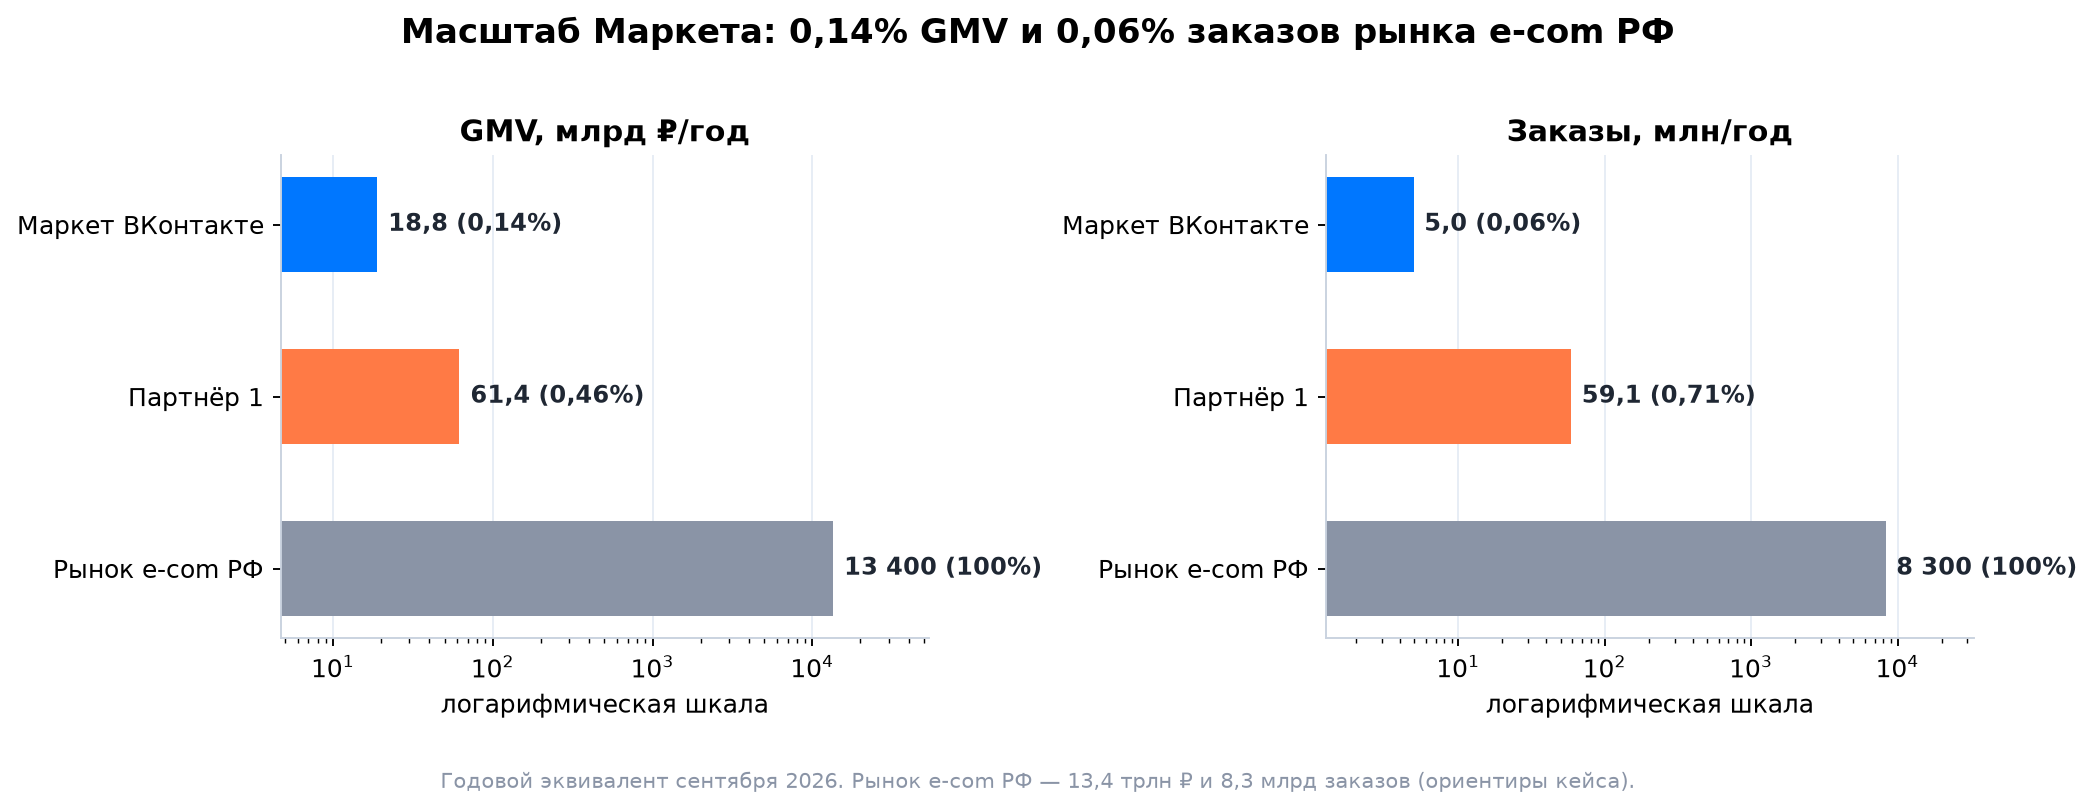
\includegraphics[width=\linewidth,height=0.70\textheight,keepaspectratio]{figures/report_market_share.png}
\caption*{Рис. 1. Масштаб Маркета: 0,14\% GMV и 0,06\% заказов рынка e-com РФ}
\end{figure}

\noindent\textbf{Масштаб внутри ВКонтакте:}\par\vspace{4pt}

\begingroup
\small
\setlength{\tabcolsep}{3pt}
\renewcommand{\arraystretch}{1.12}
\rowcolors{1}{white}{zebra}
\begin{longtable}{@{}>{\raggedright\arraybackslash}p{0.3771\linewidth}>{\raggedright\arraybackslash}p{0.1561\linewidth}>{\raggedright\arraybackslash}p{0.4422\linewidth}@{}}
\rowcolor{blue}
\textcolor{white}{\textbf{Метрика}} & \textcolor{white}{\textbf{Значение}} & \textcolor{white}{\textbf{Комментарий}} \\
\endfirsthead
\rowcolor{blue}
\textcolor{white}{\textbf{Метрика}} & \textcolor{white}{\textbf{Значение}} & \textcolor{white}{\textbf{Комментарий}} \\
\endhead
\hline
DAU Маркета & 127,4 тыс. & 0,14\% от DAU ВКонтакте 90,8 млн \\
MAU Маркета & 3,0 млн & — \\
DAU/MAU & 4,3\% & низкая частота возврата \\
Видели товары за 30 дней & 66,6 млн & витрина/карточки по всей платформе \\
Открывали карточку за 30 дней & 27,3 млн & 41\% увидевших \\
Запросы в товарном поиске & 28,6 млн/мес & 18,4\% с открытием карточки \\
\hline
\end{longtable}
\endgroup
\vspace{4pt}

\textbf{Интерпретация.} Маркет не может быть «вторым Ozon/WB»: у него нет ни аудитории destination, ни логистики, ни ассортиментной экономики. Но у ВКонтакте есть то, чего нет у маркетплейсов: \textbf{контентный трафик, доверие к сообществам и 27 млн человек, которые уже открывают карточки}. Стратегическая роль — не «место», а \textbf{слой сделки внутри экосистемы}.\par

\noindent\textbf{Альтернативы роли Маркета:}\par\vspace{4pt}

\begingroup
\small
\setlength{\tabcolsep}{3pt}
\renewcommand{\arraystretch}{1.12}
\rowcolors{1}{white}{zebra}
\begin{longtable}{@{}>{\raggedright\arraybackslash}p{0.3251\linewidth}>{\raggedright\arraybackslash}p{0.3251\linewidth}>{\raggedright\arraybackslash}p{0.3251\linewidth}@{}}
\rowcolor{blue}
\textcolor{white}{\textbf{Альтернатива}} & \textcolor{white}{\textbf{Что говорят данные}} & \textcolor{white}{\textbf{Вердикт}} \\
\endfirsthead
\rowcolor{blue}
\textcolor{white}{\textbf{Альтернатива}} & \textcolor{white}{\textbf{Что говорят данные}} & \textcolor{white}{\textbf{Вердикт}} \\
\endhead
\hline
A. Самостоятельный маркетплейс (destination) & DAU 0,14\% от VK; DAU/MAU 4,3\%; конверсия открытие→заказ 0,21\%; 46\% трафика — категории с конверсией <0,1\%; заказы −10,7\% за месяц & \textbf{Не рекомендуется}: нет аудитории и экономики для лобовой конкуренции \\
B. Товарная инфраструктура + поиск + витрина внутри сообщества & 27,3 млн открывают карточки вне Маркета; 28,6 млн запросов; 92,7\% открытий Партнёра — из контента; узкое место «карточка→кнопка» ×13,7; не нужна своя логистика & \textbf{Рекомендуется}: превращает Маркет из места в слой (catalog + checkout + trust + search) \\
C. Полностью закрыть отдельную витрину & 79,5\% открытий Маркета — витрина/браузинг; «Главная Маркета» — 0,2\%; но поиск — 1,9\% и 28,6 млн запросов & \textbf{Частично}: закрывать «Главную как destination», сохранять поиск, заказы и профиль покупателя \\
\hline
\end{longtable}
\endgroup
\vspace{4pt}

\subsection{Сегменты: где находятся целевые бизнесы}

Сегментация — по стеку инструментов, а не по размеру или тематике. Это важно: она сразу показывает, \textbf{что уже подключено} и \textbf{чего не хватает}.\par

\begingroup
\scriptsize
\setlength{\tabcolsep}{3pt}
\renewcommand{\arraystretch}{1.12}
\rowcolors{1}{white}{zebra}
\begin{longtable}{@{}>{\raggedright\arraybackslash}p{0.3046\linewidth}>{\raggedright\arraybackslash}p{0.0448\linewidth}>{\raggedright\arraybackslash}p{0.1075\linewidth}>{\raggedright\arraybackslash}p{0.0806\linewidth}>{\raggedright\arraybackslash}p{0.1254\linewidth}>{\raggedright\arraybackslash}p{0.0538\linewidth}>{\raggedright\arraybackslash}p{0.0806\linewidth}>{\raggedright\arraybackslash}p{0.1165\linewidth}@{}}
\rowcolor{blue}
\textcolor{white}{\textbf{Сегмент}} & \textcolor{white}{\textbf{n}} & \textcolor{white}{\textbf{Доля выборки}} & \textcolor{white}{\textbf{Продающих}} & \textcolor{white}{\textbf{Заказов/бизнес}} & \textcolor{white}{\textbf{AOV, ₽}} & \textcolor{white}{\textbf{GMV, ₽}} & \textcolor{white}{\textbf{Роль}} \\
\endfirsthead
\rowcolor{blue}
\textcolor{white}{\textbf{Сегмент}} & \textcolor{white}{\textbf{n}} & \textcolor{white}{\textbf{Доля выборки}} & \textcolor{white}{\textbf{Продающих}} & \textcolor{white}{\textbf{Заказов/бизнес}} & \textcolor{white}{\textbf{AOV, ₽}} & \textcolor{white}{\textbf{GMV, ₽}} & \textcolor{white}{\textbf{Роль}} \\
\endhead
\hline
S0. Услуги без каталога & 1 626 & 16,7\% & 0,0\% & 0,00 & — & 0 & вне фокуса \\
S1. Контент/переписка без товаров & 2 071 & 21,2\% & 0,34\% & 0,01 & 7 071 & 91 920 & вне фокуса \\
S2. Чекаут без каталога (аномалия) & 2 096 & 21,5\% & 0,29\% & 0,003 & 2 291 & 16 040 & быстрый охват \\
S3. Витрина без чекаута & 320 & 3,3\% & 2,19\% & 0,10 & 11 306 & 361 780 & quick win \\
\textbf{S4. Каталог + чекаут} & \textbf{2 922} & \textbf{30,0\%} & \textbf{5,30\%} & \textbf{0,62} & \textbf{2 323} & \textbf{4 234 339} & \textbf{ядро} \\
S5. Каталог + чекаут + доставка & 625 & 6,4\% & 17,12\% & 2,14 & 3 308 & 4 420 108 & рост объёма \\
S6. Полный стек (+оплата) & 94 & 1,0\% & 17,02\% & 2,84 & 3 179 & 848 840 & масштаб \\
\hline
\end{longtable}
\endgroup
\vspace{4pt}

\begin{figure}[htbp]
\centering
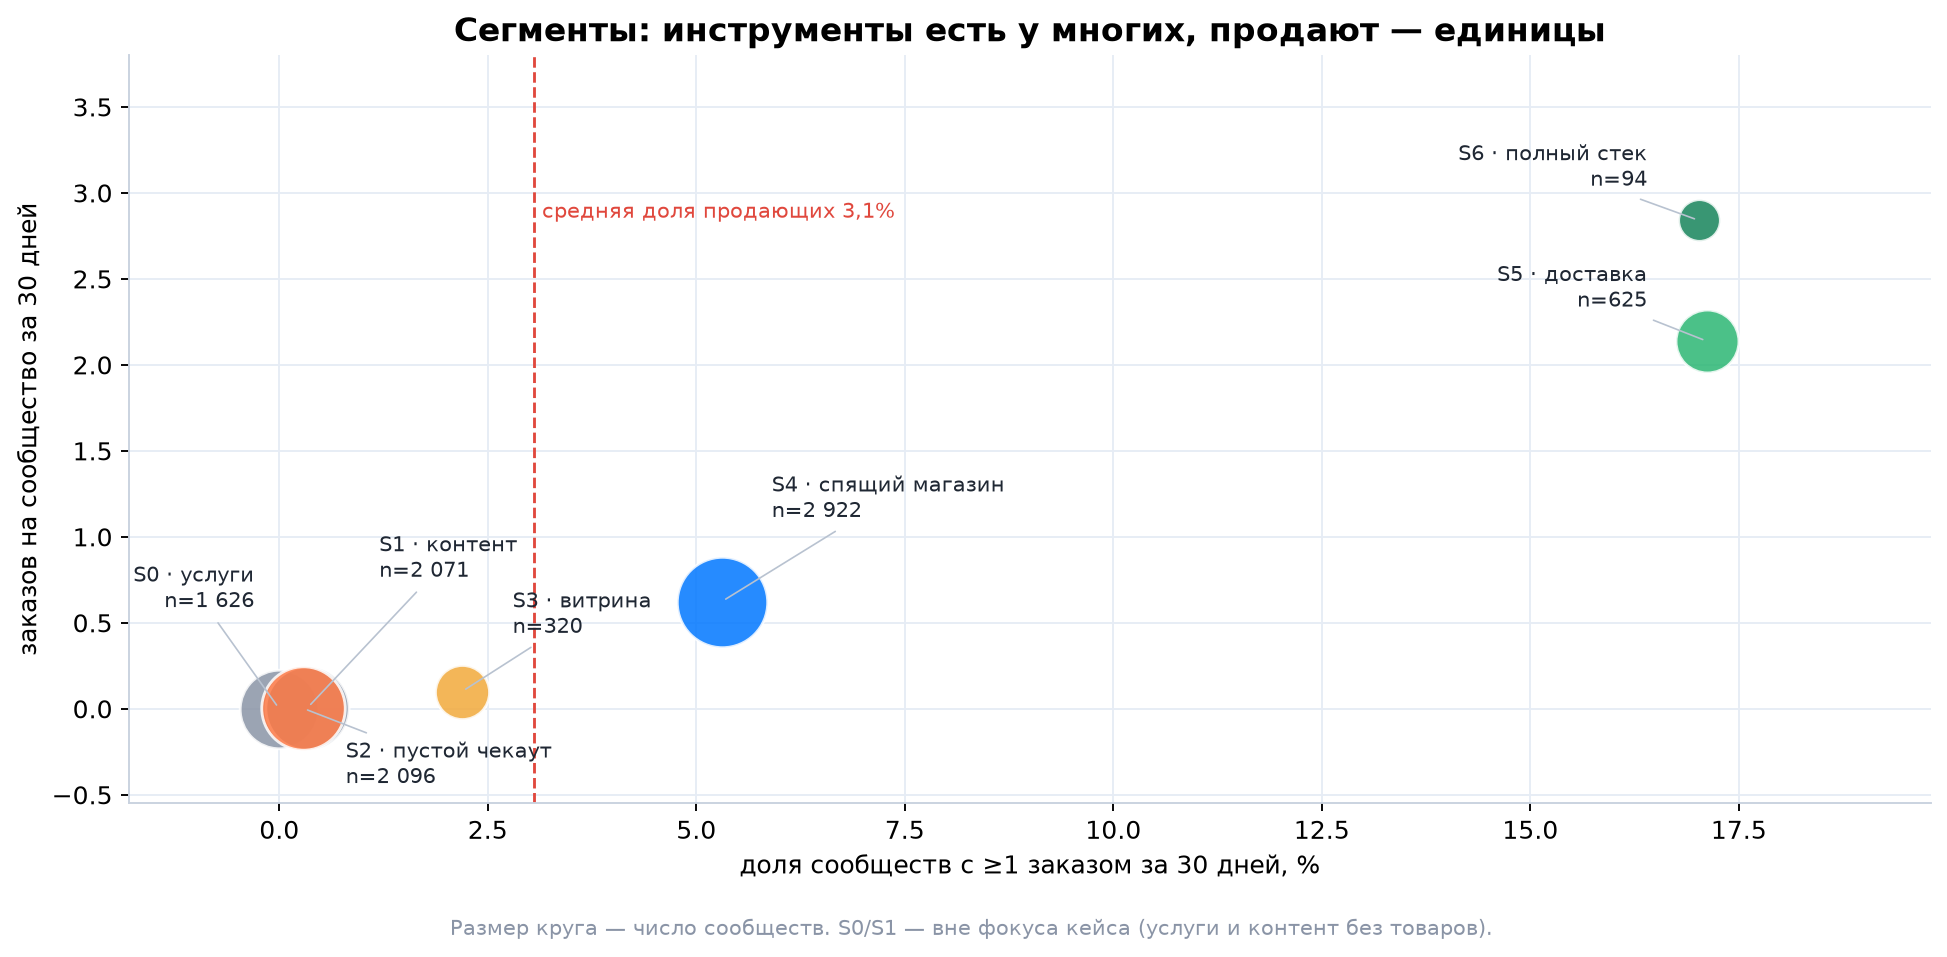
\includegraphics[width=\linewidth,height=0.70\textheight,keepaspectratio]{figures/report_segments_map.png}
\caption*{Рис. 2. Сегменты: инструменты есть у многих, продают — единицы}
\end{figure}

\noindent\textbf{Что видно:}\par\vspace{4pt}

\begin{itemize}[leftmargin=1.35em,itemsep=2pt,topsep=3pt,parsep=0pt]
\item \textbf{S4 — 30\% выборки, но только 5,3\% продающих.} У них есть каталог (медиана 9 SKU) и чекаут, но нет доставки. Это самый большой адресуемый сегмент: 2 922 сообщества.
\item \textbf{S2 — 2 096 сообществ с «пустым чекаутом».} Технически это аномалия, но с точки зрения бизнеса — это люди, которые уже нажали «подключить продажи», но не наполнили каталог. Быстрый прирост даёт импорт каталога.
\item \textbf{S5/S6 — 719 сообществ, 17\% продающих.} Они уже продают; им нужен новый трафик, повторные покупки и монетизация, а не «ещё один чекаут».
\item \textbf{S3 — 320 сообществ, витрина без чекаута.} Быстрый win: включить чекаут по умолчанию.
\item \textbf{S0/S1 — 3 697 сообществ (38\%).} Услуги и контент без товаров; кейс просит сфокусироваться на товарах, поэтому в первый год не тратим на них ресурс.
\end{itemize}

\noindent\textbf{Портреты целевых сегментов:}\par\vspace{4pt}

\begingroup
\footnotesize
\setlength{\tabcolsep}{3pt}
\renewcommand{\arraystretch}{1.12}
\rowcolors{1}{white}{zebra}
\begin{longtable}{@{}>{\raggedright\arraybackslash}p{0.1246\linewidth}>{\raggedright\arraybackslash}p{0.2123\linewidth}>{\raggedright\arraybackslash}p{0.1892\linewidth}>{\raggedright\arraybackslash}p{0.2123\linewidth}>{\raggedright\arraybackslash}p{0.2123\linewidth}@{}}
\rowcolor{blue}
\textcolor{white}{\textbf{Сегмент}} & \textcolor{white}{\textbf{Профиль из данных}} & \textcolor{white}{\textbf{Цель бизнеса}} & \textcolor{white}{\textbf{Барьер}} & \textcolor{white}{\textbf{Что даём}} \\
\endfirsthead
\rowcolor{blue}
\textcolor{white}{\textbf{Сегмент}} & \textcolor{white}{\textbf{Профиль из данных}} & \textcolor{white}{\textbf{Цель бизнеса}} & \textcolor{white}{\textbf{Барьер}} & \textcolor{white}{\textbf{Что даём}} \\
\endhead
\hline
S4 «Спящий магазин» & каталог \textasciitilde{}9 SKU, 665 подписчиков, чекаут есть, доставки нет & заказы без своего сайта и логистики & не может исполнить заказ: доставка/оплата не подключены; карточка не ведёт к сделке & доставка «из коробки» + оплата + автогенерация карточек; обучение в 3 шага \\
S3 «Витрина-каталог» & каталог \textasciitilde{}20 SKU, 1 300 подписчиков, чекаута нет & показывать ассортимент и получать заявки & сделка уходит в сообщения, теряется конверсия и учёт & чекаут по умолчанию + шаблоны ответов с карточкой \\
S2 «Пустой чекаут» & чекаут подключён, каталог пуст, 280 подписчиков & попробовать продажи без затрат & нет наполненного каталога & импорт из маркетплейса/CSV, карточка из фото \\
S5/S6 «Работающий продавец» & 39–59 SKU, 1 000–1 250 подписчиков, доставка есть & масштабировать заказы и повторные покупки & мало нового трафика; товарный контент не даёт переходов & шопсы + реклама на карточку + рефералка + оплата внутри VK \\
\hline
\end{longtable}
\endgroup
\vspace{4pt}

\subsection{Воронка активации: инструмент ≠ сделка}

Вложенная воронка торгового стека:\par

\begingroup
\small
\setlength{\tabcolsep}{3pt}
\renewcommand{\arraystretch}{1.12}
\rowcolors{1}{white}{zebra}
\begin{longtable}{@{}>{\raggedright\arraybackslash}p{0.4743\linewidth}>{\raggedright\arraybackslash}p{0.0719\linewidth}>{\raggedright\arraybackslash}p{0.1725\linewidth}>{\raggedright\arraybackslash}p{0.2444\linewidth}@{}}
\rowcolor{blue}
\textcolor{white}{\textbf{Шаг}} & \textcolor{white}{\textbf{n}} & \textcolor{white}{\textbf{Доля от всех}} & \textcolor{white}{\textbf{Шаговая конверсия}} \\
\endfirsthead
\rowcolor{blue}
\textcolor{white}{\textbf{Шаг}} & \textcolor{white}{\textbf{n}} & \textcolor{white}{\textbf{Доля от всех}} & \textcolor{white}{\textbf{Шаговая конверсия}} \\
\endhead
\hline
Бизнес-сообщество в выборке & 9 754 & 100\% & — \\
Активный каталог (≥1 товар) & 3 961 & 40,6\% & 40,6\% \\
+ подключён чекаут & 3 641 & 37,3\% & 91,9\% \\
+ подключена доставка & 719 & 7,4\% & 19,7\% \\
+ подключена оплата (полный стек) & 94 & 1,0\% & 13,1\% \\
\hline
\end{longtable}
\endgroup
\vspace{4pt}

\begin{figure}[htbp]
\centering
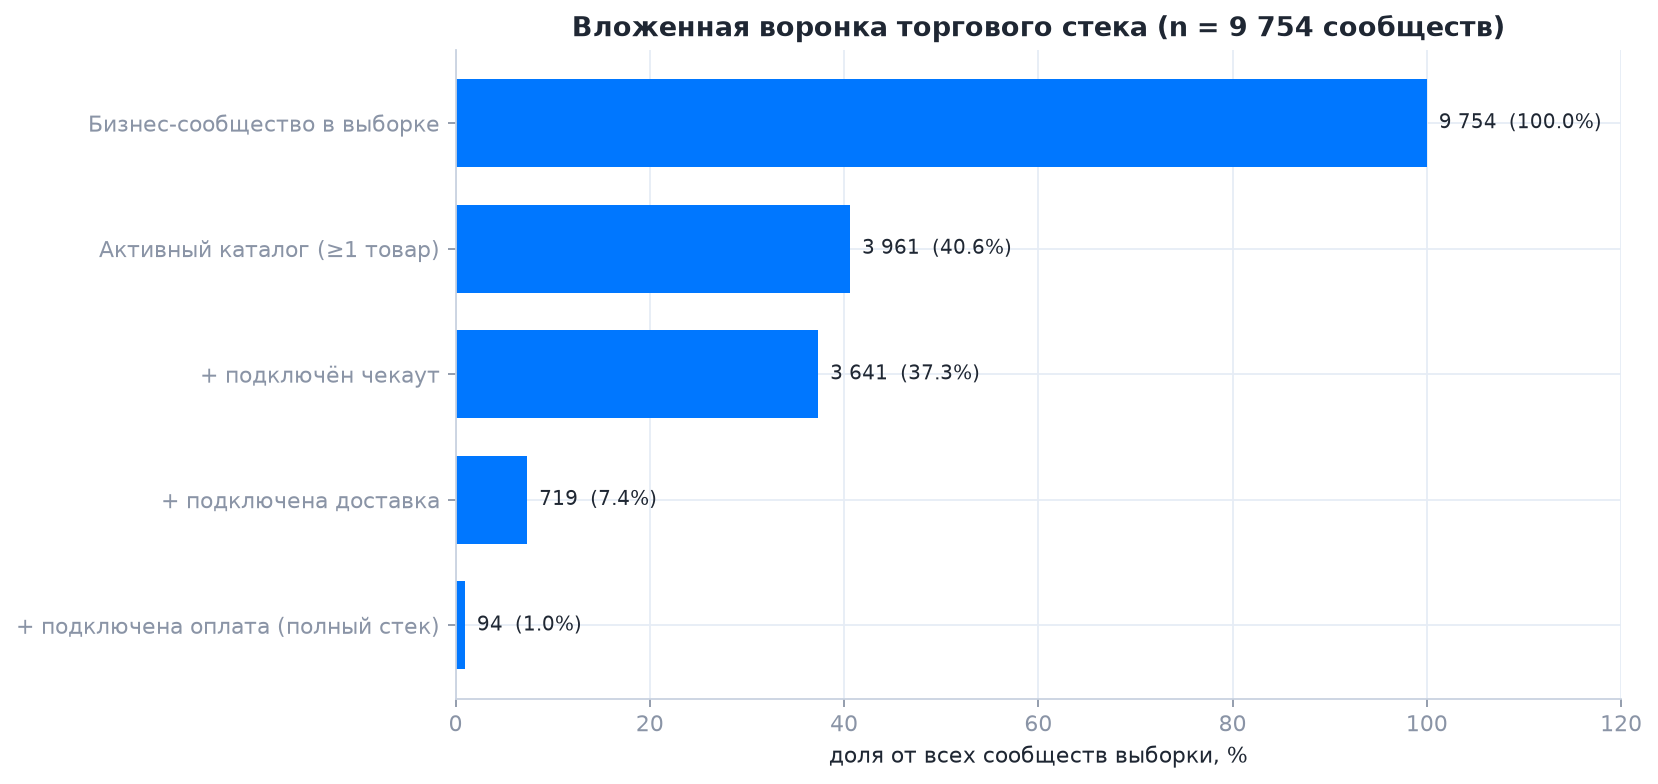
\includegraphics[width=\linewidth,height=0.70\textheight,keepaspectratio]{figures/activation_funnel.png}
\caption*{Рис. 3. Вложенная воронка торгового стека}
\end{figure}

\noindent\textbf{Ключевой разрыв — не в подключении, а в результате:}\par\vspace{4pt}

\begingroup
\small
\setlength{\tabcolsep}{3pt}
\renewcommand{\arraystretch}{1.12}
\rowcolors{1}{white}{zebra}
\begin{longtable}{@{}>{\raggedright\arraybackslash}p{0.4976\linewidth}>{\raggedright\arraybackslash}p{0.1791\linewidth}>{\raggedright\arraybackslash}p{0.2986\linewidth}@{}}
\rowcolor{blue}
\textcolor{white}{\textbf{Шаг}} & \textcolor{white}{\textbf{Сообществ}} & \textcolor{white}{\textbf{Доля от чекаута}} \\
\endfirsthead
\rowcolor{blue}
\textcolor{white}{\textbf{Шаг}} & \textcolor{white}{\textbf{Сообществ}} & \textcolor{white}{\textbf{Доля от чекаута}} \\
\endhead
\hline
Подключили чекаут & 5 737 & 100\% \\
Из них сделали ≥1 заказ & 284 & 4,95\% \\
Из них сделали ≥5 заказов & 90 & 1,57\% \\
Подключили доставку & 919 & 16,0\% \\
Подключили оплату & 255 & 4,4\% \\
\hline
\end{longtable}
\endgroup
\vspace{4pt}

\noindent\textbf{Проникновение инструментов и поведения:}\par\vspace{4pt}

\begingroup
\small
\setlength{\tabcolsep}{3pt}
\renewcommand{\arraystretch}{1.12}
\rowcolors{1}{white}{zebra}
\begin{longtable}{@{}>{\raggedright\arraybackslash}p{0.7537\linewidth}>{\raggedright\arraybackslash}p{0.1108\linewidth}>{\raggedright\arraybackslash}p{0.1108\linewidth}@{}}
\rowcolor{blue}
\textcolor{white}{\textbf{Индикатор}} & \textcolor{white}{\textbf{n}} & \textcolor{white}{\textbf{Доля}} \\
\endfirsthead
\rowcolor{blue}
\textcolor{white}{\textbf{Индикатор}} & \textcolor{white}{\textbf{n}} & \textcolor{white}{\textbf{Доля}} \\
\endhead
\hline
Подключён чекаут & 5 737 & 58,8\% \\
Товары загружены & 4 779 & 49,0\% \\
Активный каталог & 3 961 & 40,6\% \\
Подключена доставка & 919 & 9,4\% \\
Платит за рекламу & 542 & 5,6\% \\
Есть открытия карточки из контента & 437 & 4,5\% \\
Публикует товарный контент & 303 & 3,1\% \\
≥1 заказ через чекаут & 298 & 3,1\% \\
Подключена оплата & 255 & 2,6\% \\
Участвует в реферальной программе & 201 & 2,1\% \\
≥5 заказов через чекаут & 93 & 1,0\% \\
\hline
\end{longtable}
\endgroup
\vspace{4pt}

\begin{figure}[htbp]
\centering
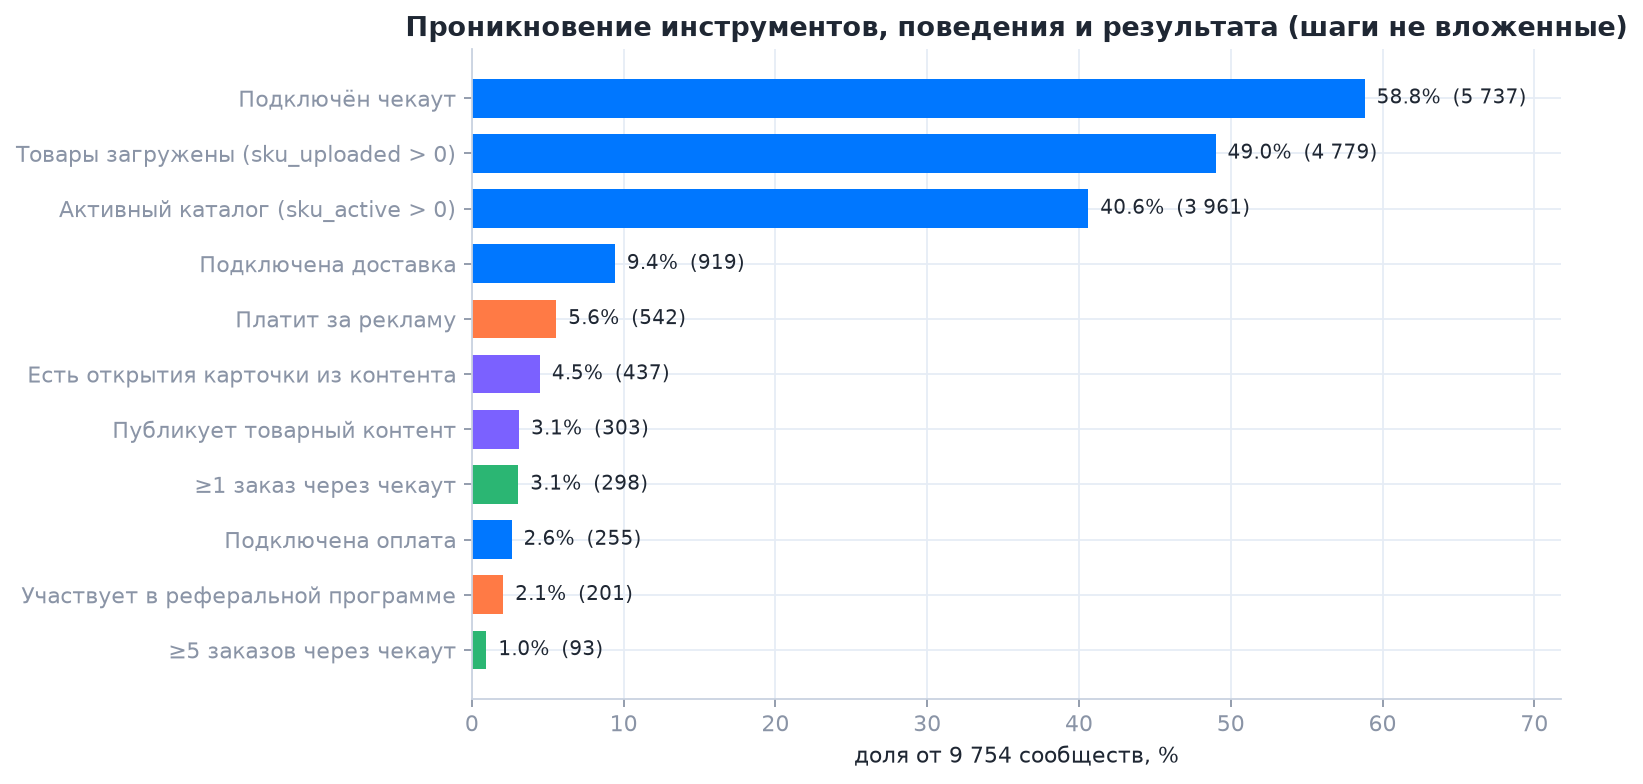
\includegraphics[width=\linewidth,height=0.70\textheight,keepaspectratio]{figures/01_penetration.png}
\caption*{Рис. 4. Проникновение инструментов, поведения и результата}
\end{figure}

\textbf{Вывод.} Проблема не в том, что бизнес не подключает инструменты: чекаут подключён у 58,8\%. Проблема в том, что \textbf{подключение не превращается в сделку}. Это подтверждает гипотезу кейса: нужен не «ещё один инструмент», а связка «каталог → карточка → кнопка → оплата → исполнение».\par

\subsection{Что связано с первой продажей}

Логит вероятности ≥1 заказа (n=9 754):\par

\begingroup
\footnotesize
\setlength{\tabcolsep}{3pt}
\renewcommand{\arraystretch}{1.12}
\rowcolors{1}{white}{zebra}
\begin{longtable}{@{}>{\raggedright\arraybackslash}p{0.1901\linewidth}>{\raggedright\arraybackslash}p{0.0475\linewidth}>{\raggedright\arraybackslash}p{0.1188\linewidth}>{\raggedright\arraybackslash}p{0.0832\linewidth}>{\raggedright\arraybackslash}p{0.5110\linewidth}@{}}
\rowcolor{blue}
\textcolor{white}{\textbf{Признак}} & \textcolor{white}{\textbf{OR}} & \textcolor{white}{\textbf{95\% ДИ}} & \textcolor{white}{\textbf{p-value}} & \textcolor{white}{\textbf{Интерпретация}} \\
\endfirsthead
\rowcolor{blue}
\textcolor{white}{\textbf{Признак}} & \textcolor{white}{\textbf{OR}} & \textcolor{white}{\textbf{95\% ДИ}} & \textcolor{white}{\textbf{p-value}} & \textcolor{white}{\textbf{Интерпретация}} \\
\endhead
\hline
checkout & 8,27 & 3,69–18,54 & <0,001 & тавтологичен: без чекаута нет заказа \\
delivery & 1,59 & 1,18–2,14 & 0,002 & связано с более высокой активацией \\
log\_sku & 1,52 & 1,39–1,65 & <0,001 & каждый e× каталога — +52\% к шансу \\
log\_views\_reg & 1,45 & 1,30–1,61 & <0,001 & охват важен \\
has\_prod\_content & 1,51 & 0,96–2,36 & 0,073 & на грани значимости \\
log\_subs & 1,19 & 1,07–1,33 & 0,002 & размер аудитории \\
payment & 1,14 & 0,71–1,82 & 0,60 & эффект не выделяется \\
referral & 1,14 & 0,60–2,16 & 0,69 & мало данных \\
log\_ad\_spend & 1,02 & 0,98–1,06 & 0,31 & связи с первой продажей нет \\
log\_content & 0,81 & 0,70–0,92 & 0,002 & больше постов без каталога — ниже активация \\
\hline
\end{longtable}
\endgroup
\vspace{4pt}

\begin{figure}[htbp]
\centering
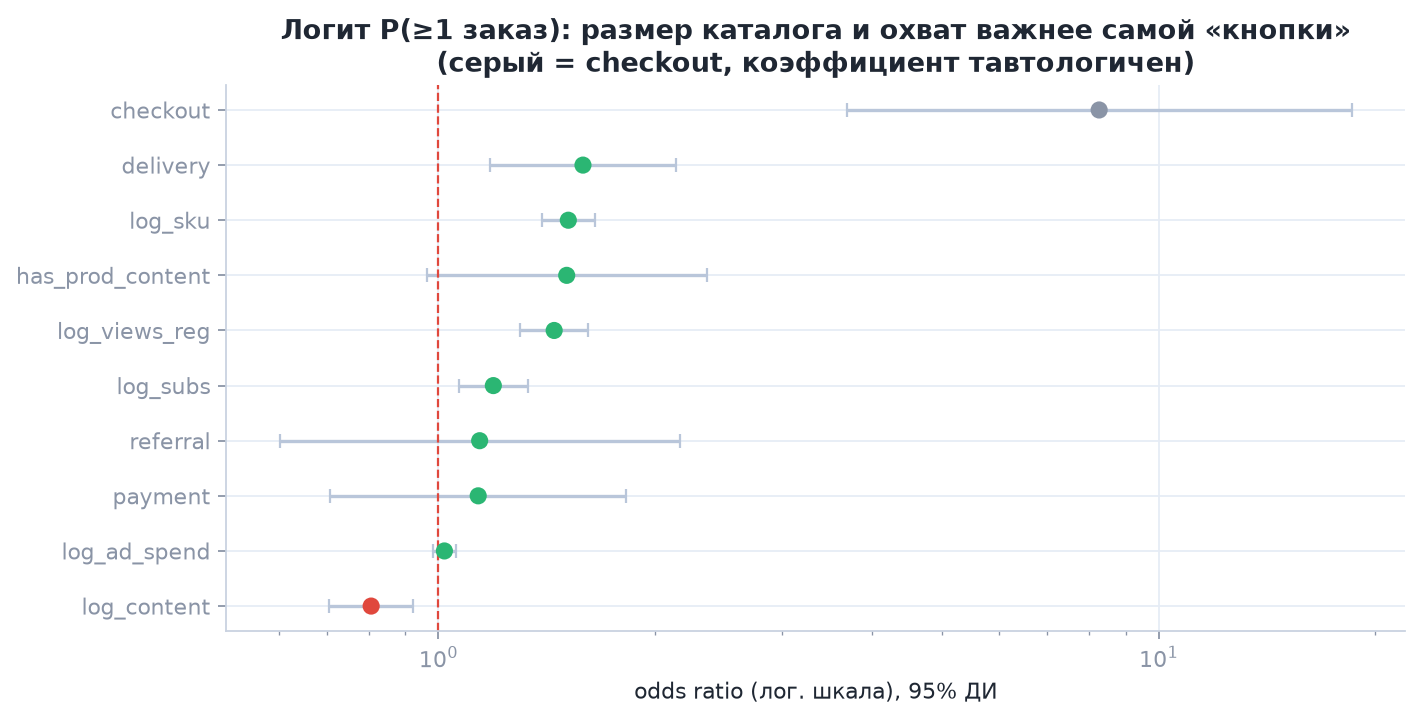
\includegraphics[width=\linewidth,height=0.70\textheight,keepaspectratio]{figures/02_logit_forest.png}
\caption*{Рис. 5. Логит: размер каталога и охват важнее «кнопки»}
\end{figure}

ML-модель (AUC 0,84, AP 0,39) ставит \textbf{размер активного каталога} на первое место по важности. Это не причинный эффект, но сильный сигнал: \textbf{ассортимент — первый экран онбординга}, а не «настройка кнопки».\par

\subsection{Доставка: наивный разрыв и PSM}

Наивное сравнение: S5 (с доставкой) — 17,1\% продающих, S4 (без доставки) — 5,3\%; отношение \textbf{×3,2}, разница \textbf{+11,8 п.п.} (95\% ДИ 8,9–15,1; p<0,001).\par

Но S5 и S4 различаются не только доставкой:\par

\begingroup
\small
\setlength{\tabcolsep}{3pt}
\renewcommand{\arraystretch}{1.12}
\rowcolors{1}{white}{zebra}
\begin{longtable}{@{}>{\raggedright\arraybackslash}p{0.7444\linewidth}>{\raggedright\arraybackslash}p{0.1027\linewidth}>{\raggedright\arraybackslash}p{0.1283\linewidth}@{}}
\rowcolor{blue}
\textcolor{white}{\textbf{Показатель}} & \textcolor{white}{\textbf{S4}} & \textcolor{white}{\textbf{S5}} \\
\endfirsthead
\rowcolor{blue}
\textcolor{white}{\textbf{Показатель}} & \textcolor{white}{\textbf{S4}} & \textcolor{white}{\textbf{S5}} \\
\endhead
\hline
Медиана подписчиков & 665 & 1 000 \\
Медиана активных SKU & 9 & 39 \\
Медиана публикаций за 30 дней & 3 & 5 \\
Доля с товарным контентом & 3,7\% & 12,5\% \\
Доля продающих & 5,3\% & 17,1\% \\
\hline
\end{longtable}
\endgroup
\vspace{4pt}

После PSM по наблюдаемым признакам:\par

\begingroup
\footnotesize
\setlength{\tabcolsep}{3pt}
\renewcommand{\arraystretch}{1.12}
\rowcolors{1}{white}{zebra}
\begin{longtable}{@{}>{\raggedright\arraybackslash}p{0.1995\linewidth}>{\raggedright\arraybackslash}p{0.2347\linewidth}>{\raggedright\arraybackslash}p{0.2582\linewidth}>{\raggedright\arraybackslash}p{0.1056\linewidth}>{\raggedright\arraybackslash}p{0.1526\linewidth}@{}}
\rowcolor{blue}
\textcolor{white}{\textbf{Outcome}} & \textcolor{white}{\textbf{Наивно}} & \textcolor{white}{\textbf{После PSM}} & \textcolor{white}{\textbf{ATT}} & \textcolor{white}{\textbf{95\% ДИ}} \\
\endfirsthead
\rowcolor{blue}
\textcolor{white}{\textbf{Outcome}} & \textcolor{white}{\textbf{Наивно}} & \textcolor{white}{\textbf{После PSM}} & \textcolor{white}{\textbf{ATT}} & \textcolor{white}{\textbf{95\% ДИ}} \\
\endhead
\hline
Доля продающих & 17,1\% vs 5,3\% (×3,2) & 16,7\% vs 13,4\% (×1,24) & \textbf{+3,2 п.п.} & \textbf{−0,4…+7,1} \\
Заказов на бизнес & 2,23 vs 0,62 & 2,20 vs 2,79 & −0,60 & −2,71…+1,24 \\
GMV на бизнес, ₽ & 7 328 vs 1 449 & 7 019 vs 5 715 & +1 304 & −2 885…+5 834 \\
\hline
\end{longtable}
\endgroup
\vspace{4pt}

\begin{figure}[htbp]
\centering
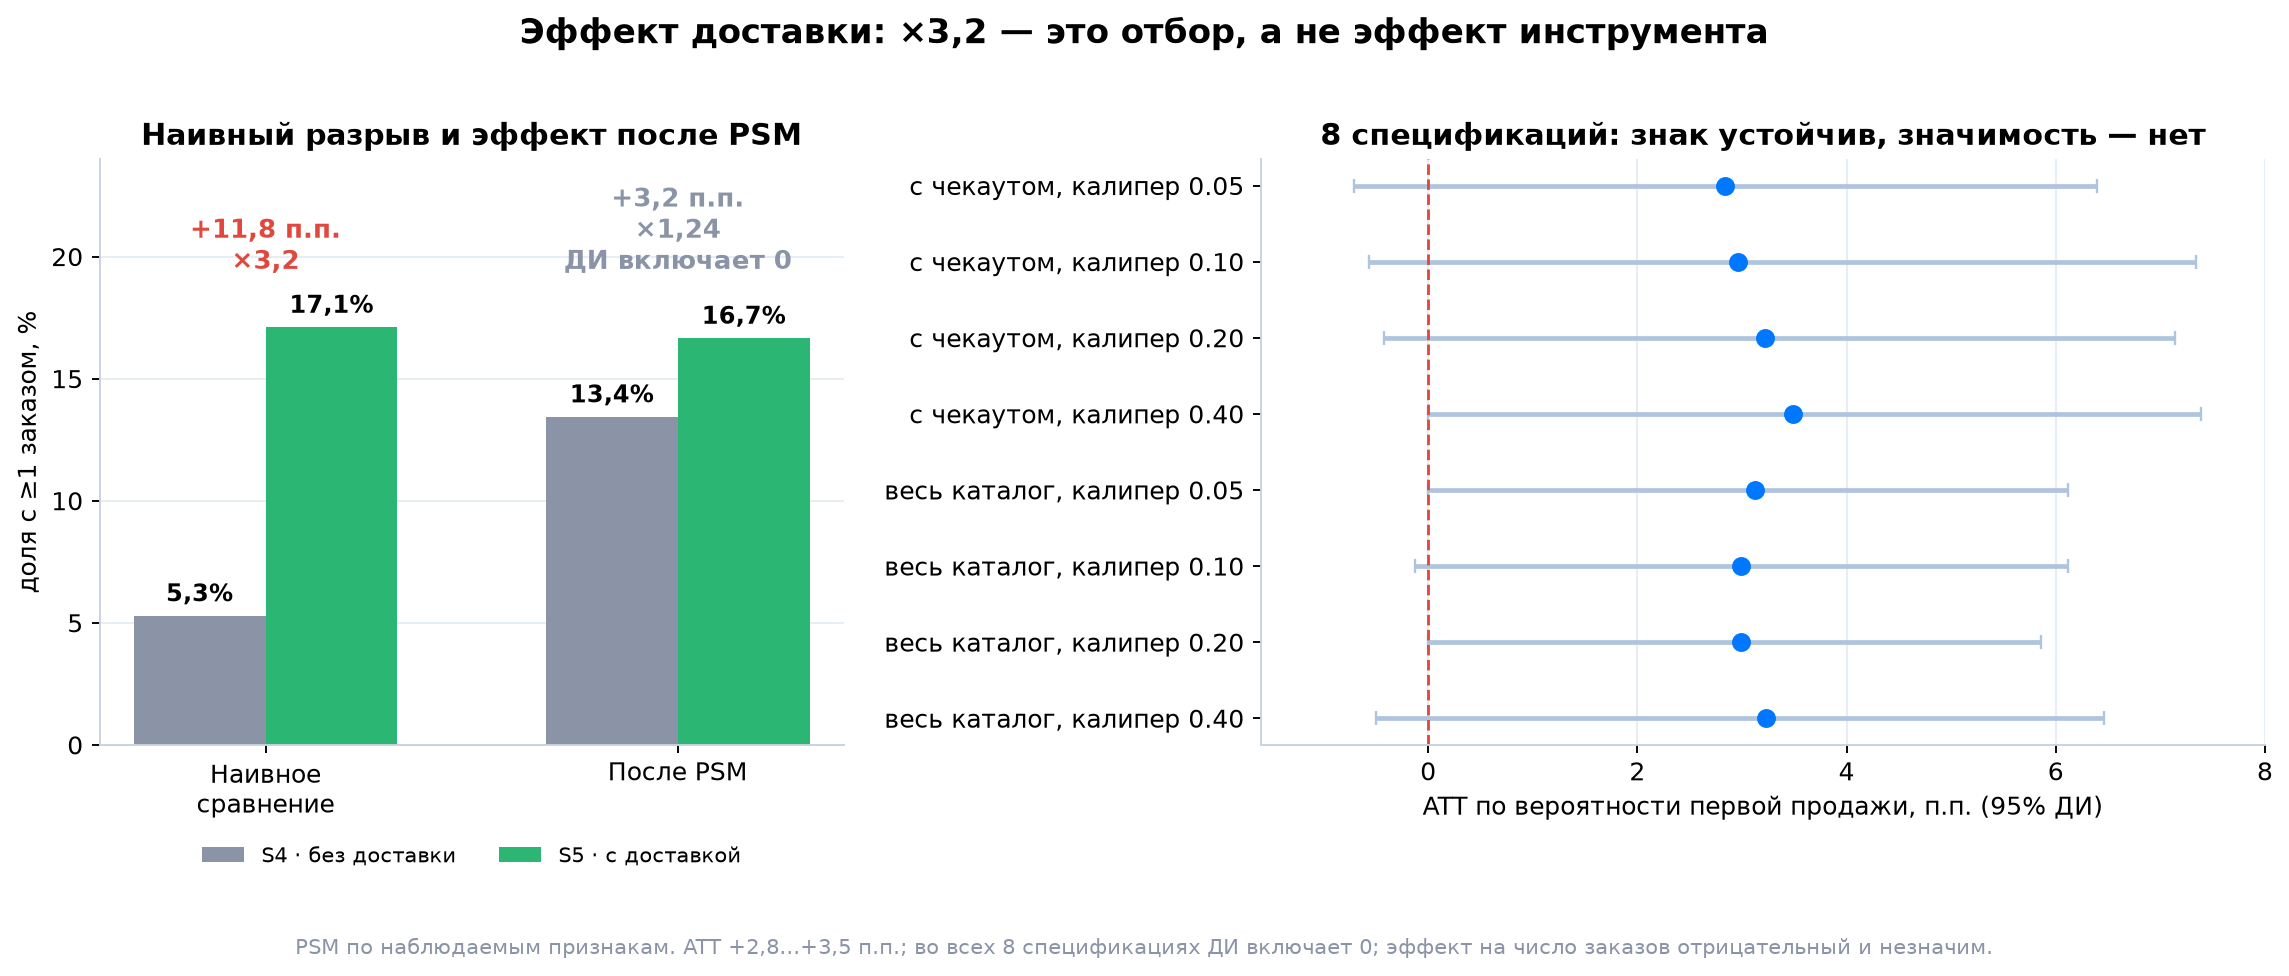
\includegraphics[width=\linewidth,height=0.70\textheight,keepaspectratio]{figures/report_psm.png}
\caption*{Рис. 6. Эффект доставки: ×3,2 — это отбор, а не эффект инструмента}
\end{figure}

В 8 спецификациях PSM (2 контроля × 4 калипера) ATT активации — \textbf{+2,8…+3,5 п.п.}, но \textbf{во всех 8 ДИ включает 0}; эффект на число заказов — \textbf{−0,3…−1,1} и незначим. Это важнейший результат для честности презентации: \textbf{доставка — необходимый, но не достаточный элемент}. Она снимает барьер исполнения, но не создаёт спрос и ассортимент.\par

\subsection{Товарный контент: охват есть, конверсии нет}

\begingroup
\small
\setlength{\tabcolsep}{3pt}
\renewcommand{\arraystretch}{1.12}
\rowcolors{1}{white}{zebra}
\begin{longtable}{@{}>{\raggedright\arraybackslash}p{0.7322\linewidth}>{\raggedright\arraybackslash}p{0.2554\linewidth}@{}}
\rowcolor{blue}
\textcolor{white}{\textbf{Показатель}} & \textcolor{white}{\textbf{Значение}} \\
\endfirsthead
\rowcolor{blue}
\textcolor{white}{\textbf{Показатель}} & \textcolor{white}{\textbf{Значение}} \\
\endhead
\hline
Публикаций всего & 199 079 \\
Публикаций с товаром & 17 946 (9,0\%) \\
Просмотров обычного контента & 316,2 млн \\
Просмотров товарного контента & 18,4 млн (5,5\%) \\
Сообществ, публикующих товарный контент & 303 (3,1\%) \\
Сообществ с открытиями карточки из контента & 437 (4,5\%) \\
CTR товарного контента в карточку & \textbf{0,29\%} \\
\hline
\end{longtable}
\endgroup
\vspace{4pt}

Парное сравнение внутри сообщества (299 пар):\par

\begingroup
\small
\setlength{\tabcolsep}{3pt}
\renewcommand{\arraystretch}{1.12}
\rowcolors{1}{white}{zebra}
\begin{longtable}{@{}>{\raggedright\arraybackslash}p{0.5645\linewidth}>{\raggedright\arraybackslash}p{0.1328\linewidth}>{\raggedright\arraybackslash}p{0.1162\linewidth}>{\raggedright\arraybackslash}p{0.1494\linewidth}@{}}
\rowcolor{blue}
\textcolor{white}{\textbf{Метрика}} & \textcolor{white}{\textbf{Товарный}} & \textcolor{white}{\textbf{Обычный}} & \textcolor{white}{\textbf{Отношение}} \\
\endfirsthead
\rowcolor{blue}
\textcolor{white}{\textbf{Метрика}} & \textcolor{white}{\textbf{Товарный}} & \textcolor{white}{\textbf{Обычный}} & \textcolor{white}{\textbf{Отношение}} \\
\endhead
\hline
Просмотров на публикацию (медиана) & 702 & 375 & \textbf{×1,90} \\
ER (медиана) & — & — & \textbf{×0,54} \\
Доля пар, где товарный хуже по ER & — & — & 72,6\% \\
\hline
\end{longtable}
\endgroup
\vspace{4pt}

\begin{figure}[htbp]
\centering
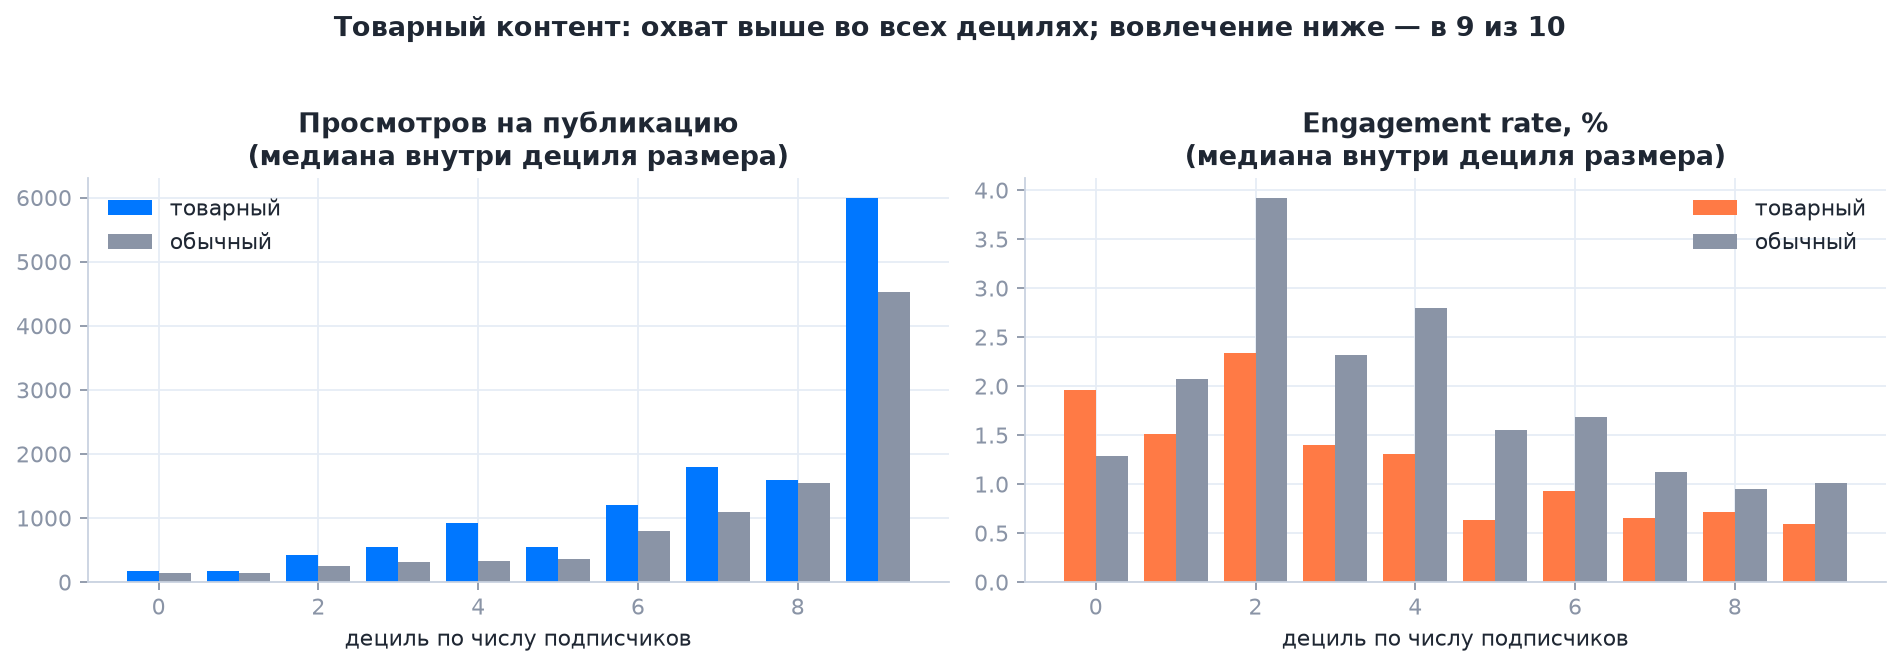
\includegraphics[width=\linewidth,height=0.70\textheight,keepaspectratio]{figures/02_content_by_decile.png}
\caption*{Рис. 7. Товарный контент: охват выше во всех децилях, вовлечение ниже}
\end{figure}

\textbf{Парадокс Симпсона:} агрегатное отношение просмотров товарного к обычному — \textbf{0,64} (крупные сообщества «тянут» вниз), а медиана парных отношений — \textbf{1,90}. Правильный вывод — \textbf{внутри сообщества товарный контент получает больше охвата}, но \textbf{меньше вовлечения}. Устойчивость: 1,90–1,97 после исключения топ-1\% и рекламы.\par

\textbf{Что это значит.} Контент — канал \textbf{дистрибуции}, а не магическая конверсия. Сам по себе товарный пост не ведёт в карточку: CTR 0,29\% — это 3 перехода на 1 000 просмотров. Нужен формат: цена, скидка, CTA, дефицит, отзыв, ссылка на карточку. И нужен повод: 3,1\% сообществ публикуют товарный контент — почти никто.\par

\subsection{Воронка Маркета vs Партнёра: где именно теряются заказы}

\begingroup
\small
\setlength{\tabcolsep}{3pt}
\renewcommand{\arraystretch}{1.12}
\rowcolors{1}{white}{zebra}
\begin{longtable}{@{}>{\raggedright\arraybackslash}p{0.3428\linewidth}>{\raggedright\arraybackslash}p{0.2612\linewidth}>{\raggedright\arraybackslash}p{0.2122\linewidth}>{\raggedright\arraybackslash}p{0.1469\linewidth}@{}}
\rowcolor{blue}
\textcolor{white}{\textbf{Шаг}} & \textcolor{white}{\textbf{Маркет ВКонтакте}} & \textcolor{white}{\textbf{Партнёр 1}} & \textcolor{white}{\textbf{Отношение}} \\
\endfirsthead
\rowcolor{blue}
\textcolor{white}{\textbf{Шаг}} & \textcolor{white}{\textbf{Маркет ВКонтакте}} & \textcolor{white}{\textbf{Партнёр 1}} & \textcolor{white}{\textbf{Отношение}} \\
\endhead
\hline
Показы товаров & 4 777 750 023 & 5 729 628 790 & 1,20 \\
Открытия карточки & 193 512 461 & 86 882 822 & 0,45 \\
Нажатия кнопки & 5 969 063 & 36 626 075 & 6,14 \\
Заказы & 413 740 & 4 927 525 & \textbf{11,91} \\
CTR показа→открытие & 4,05\% & 1,52\% & 0,37 \\
Открытие→кнопка & \textbf{3,08\%} & \textbf{42,16\%} & \textbf{13,67} \\
Кнопка→заказ & 6,93\% & 13,45\% & 1,94 \\
Открытие→заказ & \textbf{0,21\%} & \textbf{5,67\%} & \textbf{26,5} \\
AOV, ₽ & 3 781 & 1 039 & 0,27 \\
Заказов на покупателя & 1,40 & 1,70 & 1,21 \\
\hline
\end{longtable}
\endgroup
\vspace{4pt}

\begin{figure}[htbp]
\centering
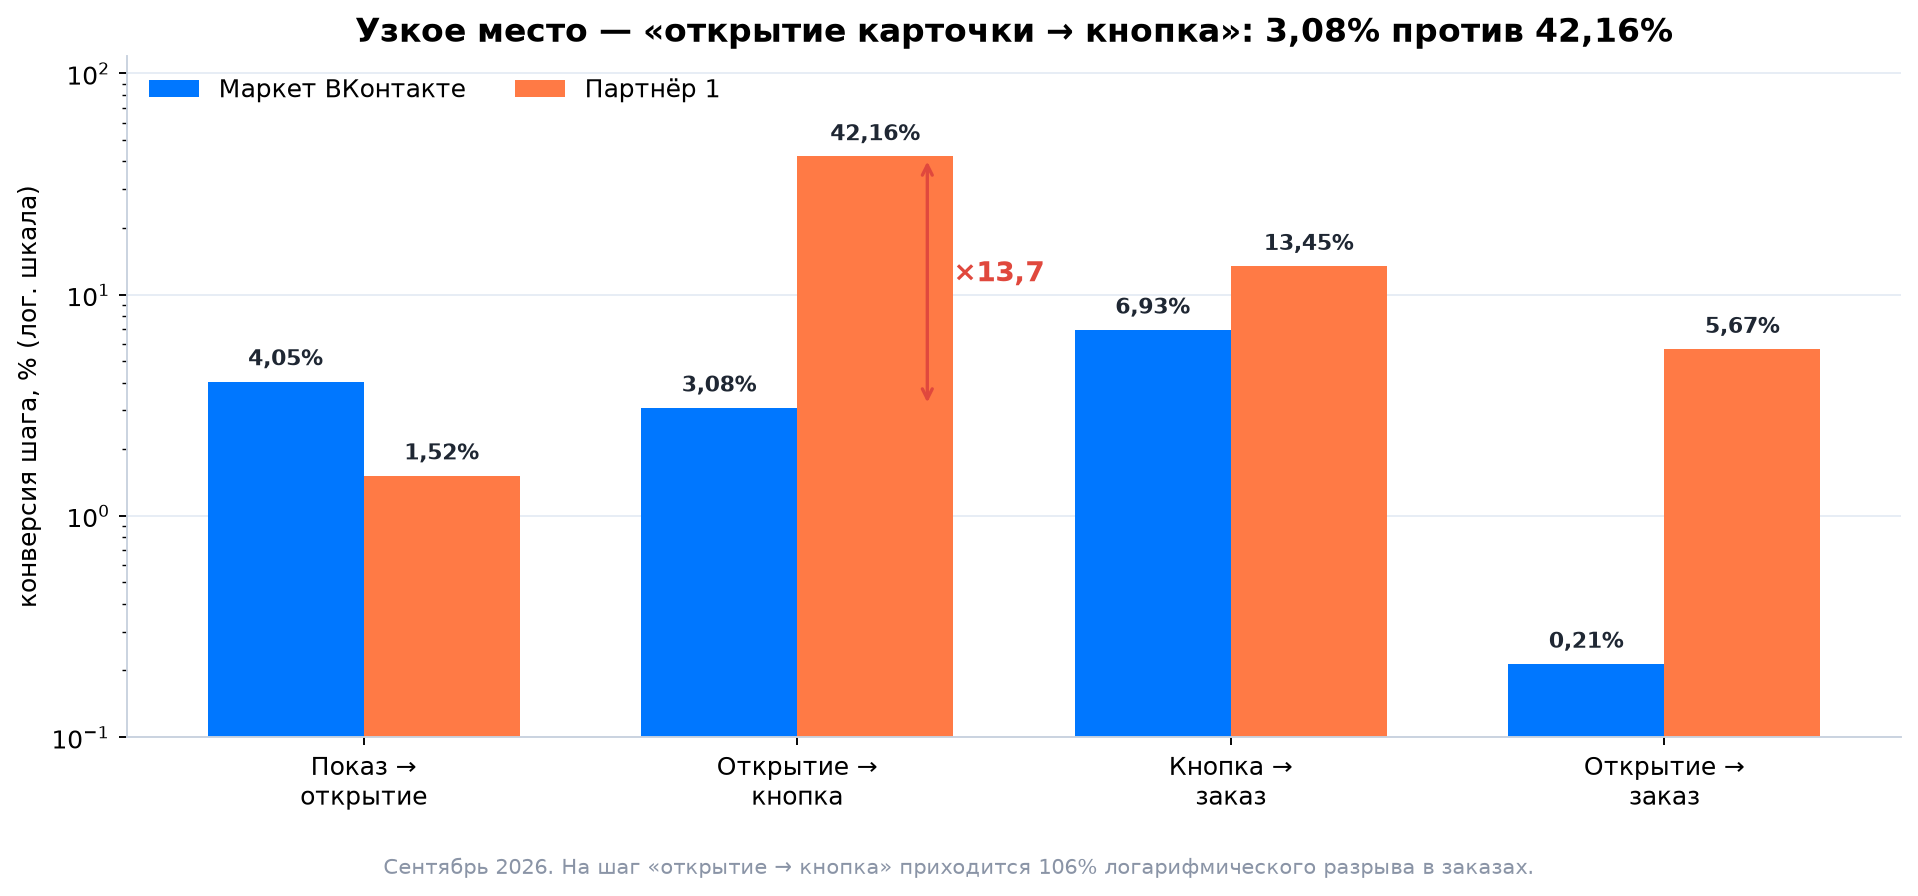
\includegraphics[width=\linewidth,height=0.70\textheight,keepaspectratio]{figures/report_funnel_compare.png}
\caption*{Рис. 8. Воронка Маркета ВКонтакте и Партнёра 1}
\end{figure}

\noindent\textbf{Декомпозиция разрыва в заказах (лог-вклады):}\par\vspace{4pt}

\begingroup
\small
\setlength{\tabcolsep}{3pt}
\renewcommand{\arraystretch}{1.12}
\rowcolors{1}{white}{zebra}
\begin{longtable}{@{}>{\raggedright\arraybackslash}p{0.8057\linewidth}>{\raggedright\arraybackslash}p{0.1819\linewidth}@{}}
\rowcolor{blue}
\textcolor{white}{\textbf{Шаг}} & \textcolor{white}{\textbf{Вклад}} \\
\endfirsthead
\rowcolor{blue}
\textcolor{white}{\textbf{Шаг}} & \textcolor{white}{\textbf{Вклад}} \\
\endhead
\hline
Показы товаров (объём трафика) & +7,3\% \\
Показ → открытие карточки (CTR) & −39,7\% \\
\textbf{Открытие → нажатие кнопки} & \textbf{+105,6\%} \\
Нажатие → заказ & +26,8\% \\
\hline
\end{longtable}
\endgroup
\vspace{4pt}

\begin{figure}[htbp]
\centering
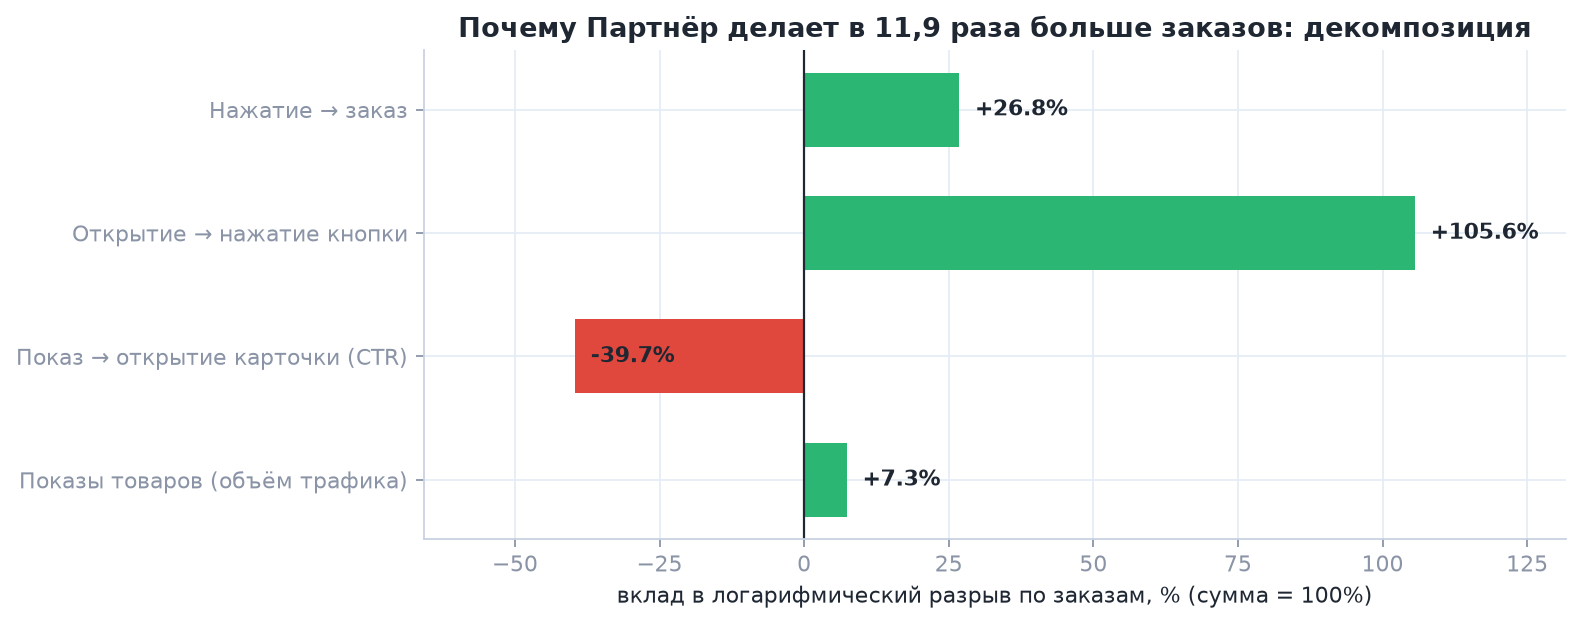
\includegraphics[width=\linewidth,height=0.70\textheight,keepaspectratio]{figures/03_gap_decomposition.png}
\caption*{Рис. 9. Почему Партнёр делает в 11,9 раза больше заказов}
\end{figure}

\noindent\textbf{Состав трафика vs механика:}\par\vspace{4pt}

\begingroup
\small
\setlength{\tabcolsep}{3pt}
\renewcommand{\arraystretch}{1.12}
\rowcolors{1}{white}{zebra}
\begin{longtable}{@{}>{\raggedright\arraybackslash}p{0.6044\linewidth}>{\raggedright\arraybackslash}p{0.1236\linewidth}>{\raggedright\arraybackslash}p{0.2473\linewidth}@{}}
\rowcolor{blue}
\textcolor{white}{\textbf{Компонента}} & \textcolor{white}{\textbf{Отношение}} & \textcolor{white}{\textbf{Вклад в лог-разрыв}} \\
\endfirsthead
\rowcolor{blue}
\textcolor{white}{\textbf{Компонента}} & \textcolor{white}{\textbf{Отношение}} & \textcolor{white}{\textbf{Вклад в лог-разрыв}} \\
\endhead
\hline
Состав трафика (какие категории смотрят) & ×0,65 & \textbf{−14\%} \\
Механика внутри категорий (карточка → заказ) & ×35,09 & \textbf{+114\%} \\
Итого (Партнёр / Маркет) & ×22,7 & 100\% \\
\hline
\end{longtable}
\endgroup
\vspace{4pt}

\begin{figure}[htbp]
\centering
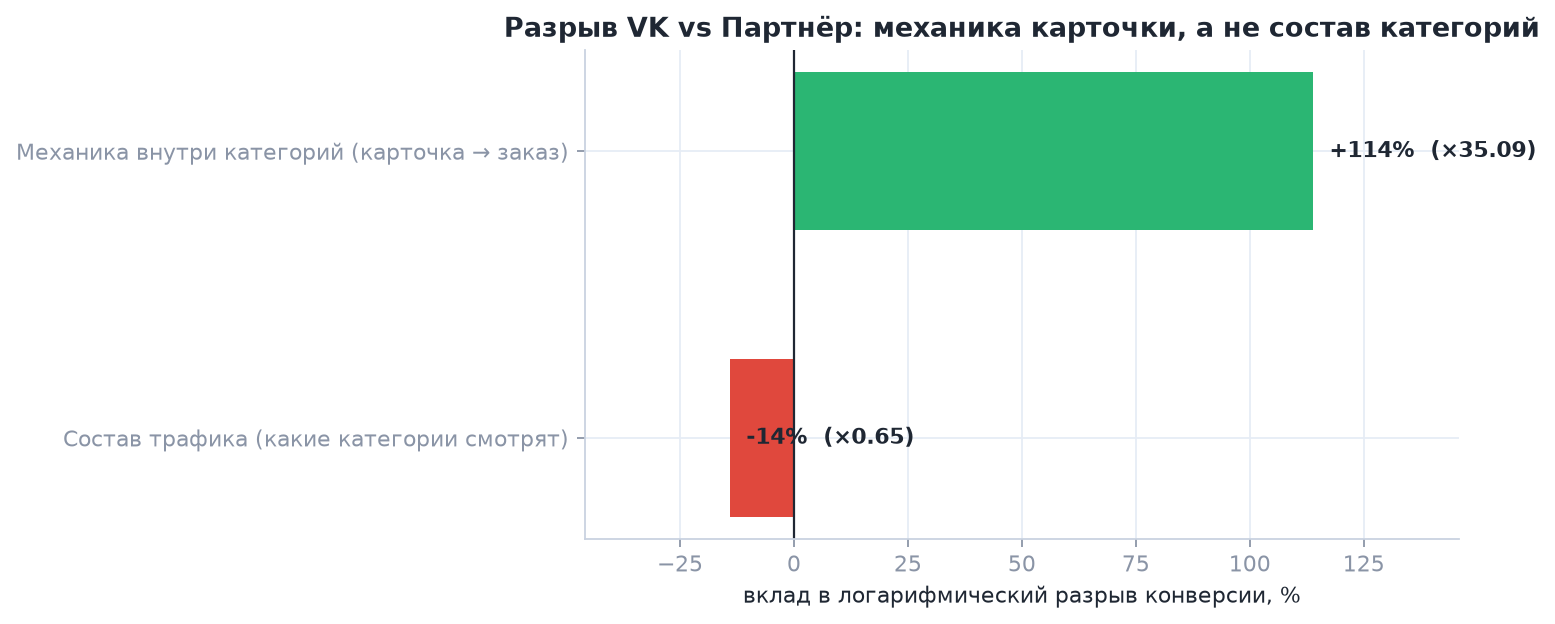
\includegraphics[width=\linewidth,height=0.70\textheight,keepaspectratio]{figures/05_gap_mix_vs_within.png}
\caption*{Рис. 10. Разрыв VK vs Партнёр: механика карточки, а не состав категорий}
\end{figure}

\textbf{Оговорка:} в разложение входят 17 категорий, где есть открытия у обоих, поэтому итоговое отношение 22,7, а не 26,5 по полным данным. На вывод о вкладе механики это не влияет.\par

\noindent\textbf{Структура источников открытий:}\par\vspace{4pt}

\begingroup
\small
\setlength{\tabcolsep}{3pt}
\renewcommand{\arraystretch}{1.12}
\rowcolors{1}{white}{zebra}
\begin{longtable}{@{}>{\raggedright\arraybackslash}p{0.3424\linewidth}>{\raggedright\arraybackslash}p{0.1284\linewidth}>{\raggedright\arraybackslash}p{0.1498\linewidth}>{\raggedright\arraybackslash}p{0.3424\linewidth}@{}}
\rowcolor{blue}
\textcolor{white}{\textbf{Источник}} & \textcolor{white}{\textbf{Маркет}} & \textcolor{white}{\textbf{Партнёр}} & \textcolor{white}{\textbf{Тип}} \\
\endfirsthead
\rowcolor{blue}
\textcolor{white}{\textbf{Источник}} & \textcolor{white}{\textbf{Маркет}} & \textcolor{white}{\textbf{Партнёр}} & \textcolor{white}{\textbf{Тип}} \\
\endhead
\hline
Другое & 40,2\% & 6,2\% & витрина/браузинг \\
Витрина магазина & 39,1\% & 0,8\% & витрина/браузинг \\
Лента & 9,7\% & 18,0\% & контент \\
Клипы & 8,9\% & 74,7\% & контент \\
Поиск & 1,9\% & 0,2\% & интент \\
Главная Маркета & 0,2\% & 0,1\% & витрина \\
\hline
\end{longtable}
\endgroup
\vspace{4pt}

\begin{figure}[htbp]
\centering
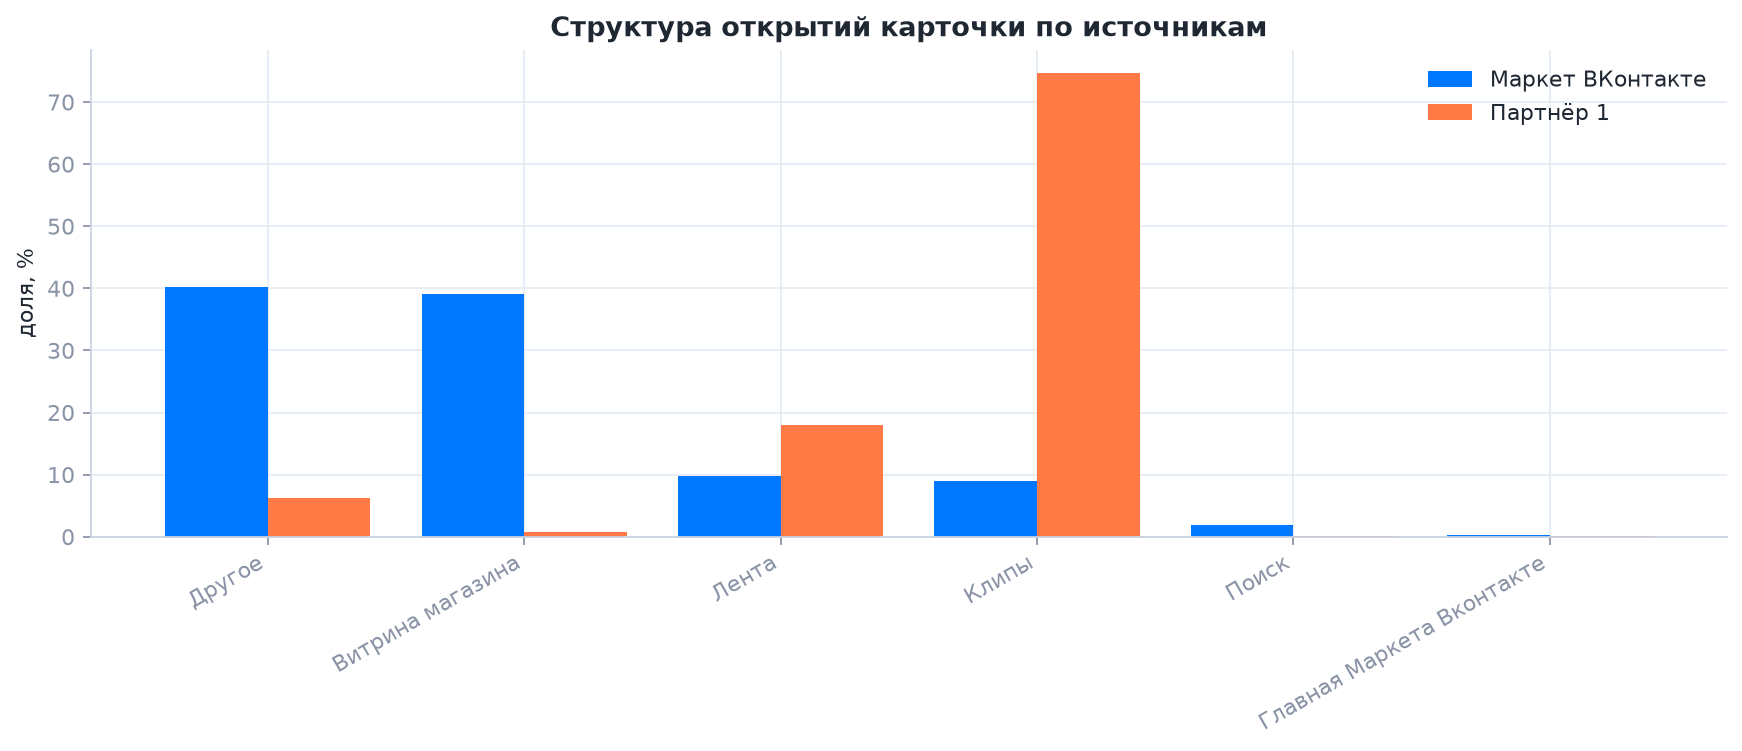
\includegraphics[width=\linewidth,height=0.70\textheight,keepaspectratio]{figures/03_sources.png}
\caption*{Рис. 11. Структура открытий карточки по источникам}
\end{figure}

\textbf{Интерпретация.} У Партнёра \textbf{92,7\%} открытий — из контента (Клипы + Лента), у Маркета — \textbf{18,6\%}, зато \textbf{79,5\%} — витрина/браузинг. Это не значит, что Маркету нужно копировать Партнёра: у Партнёра другая модель (реферальные посты и клипы). Но это доказывает, что \textbf{контентный трафик умеет продавать на той же платформе}, если карточка доводит до кнопки.\par

\textbf{Ещё один слой — «мёртвый трафик»:} 46,3\% открытий Маркета приходятся на категории с конверсией <0,1\%, но дают только 11,0\% заказов. Это не объясняет низкую конверсию (механика хуже внутри каждой категории), но объясняет, почему абсолютные заказы низкие: много показов в «Гардеробе», «Хобби», «Другое», «Дом и дача» — и мало сделок.\par

\subsection{Реклама: парадокс монетизации}

\begingroup
\small
\setlength{\tabcolsep}{3pt}
\renewcommand{\arraystretch}{1.12}
\rowcolors{1}{white}{zebra}
\begin{longtable}{@{}>{\raggedright\arraybackslash}p{0.7454\linewidth}>{\raggedright\arraybackslash}p{0.2423\linewidth}@{}}
\rowcolor{blue}
\textcolor{white}{\textbf{Показатель}} & \textcolor{white}{\textbf{Значение}} \\
\endfirsthead
\rowcolor{blue}
\textcolor{white}{\textbf{Показатель}} & \textcolor{white}{\textbf{Значение}} \\
\endhead
\hline
Платят за рекламу & 542 (5,6\%) \\
Из них без измеримого заказа & 501 (\textbf{92,4\%}) \\
Доля бюджета у «без заказа» & \textbf{87,6\%} \\
ROAS по GMV через чекаут (нижняя оценка) & \textbf{0,26} \\
OR рекламных трат в логите & 1,02 (p=0,31) \\
\hline
\end{longtable}
\endgroup
\vspace{4pt}

\textbf{Что это значит.} Реклама остаётся основным источником выручки, но \textbf{бизнес не видит результата}: 92\% плательщиков не получают измеримого заказа, а связь трат с первой продажей не значима. Это не аргумент «отключить рекламу», это аргумент \textbf{перевести её в измеримый результат}: цель кампании «заказ в чекауте», атрибуция, ROAS, удержание рекламодателя. Иначе модель «продаём трафик» будет упираться в отток.\par

\subsection{Тренды: Маркет падает, Партнёр растёт}

После поправки на день недели (30 дней, HAC-ошибки):\par

\begingroup
\footnotesize
\setlength{\tabcolsep}{3pt}
\renewcommand{\arraystretch}{1.12}
\rowcolors{1}{white}{zebra}
\begin{longtable}{@{}>{\raggedright\arraybackslash}p{0.3803\linewidth}>{\raggedright\arraybackslash}p{0.1755\linewidth}>{\raggedright\arraybackslash}p{0.1609\linewidth}>{\raggedright\arraybackslash}p{0.1463\linewidth}>{\raggedright\arraybackslash}p{0.0878\linewidth}@{}}
\rowcolor{blue}
\textcolor{white}{\textbf{Метрика}} & \textcolor{white}{\textbf{Темп, \%/день}} & \textcolor{white}{\textbf{95\% ДИ}} & \textcolor{white}{\textbf{За 30 дней}} & \textcolor{white}{\textbf{p}} \\
\endfirsthead
\rowcolor{blue}
\textcolor{white}{\textbf{Метрика}} & \textcolor{white}{\textbf{Темп, \%/день}} & \textcolor{white}{\textbf{95\% ДИ}} & \textcolor{white}{\textbf{За 30 дней}} & \textcolor{white}{\textbf{p}} \\
\endhead
\hline
Заказы: Маркет & \textbf{−0,48} & −0,83…−0,13 & \textbf{−13,4\%} & 0,008 \\
GMV: Маркет & −0,35 & −0,58…−0,11 & −9,9\% & 0,004 \\
Заказы: Партнёр & \textbf{+0,73} & +0,28…+1,19 & \textbf{+24,5\%} & 0,002 \\
GMV: Партнёр & +1,77 & +1,56…+1,99 & +69,4\% & <0,001 \\
Открытия карточки: Партнёр & +0,54 & +0,14…+0,95 & +17,6\% & 0,009 \\
\hline
\end{longtable}
\endgroup
\vspace{4pt}

\begin{figure}[htbp]
\centering
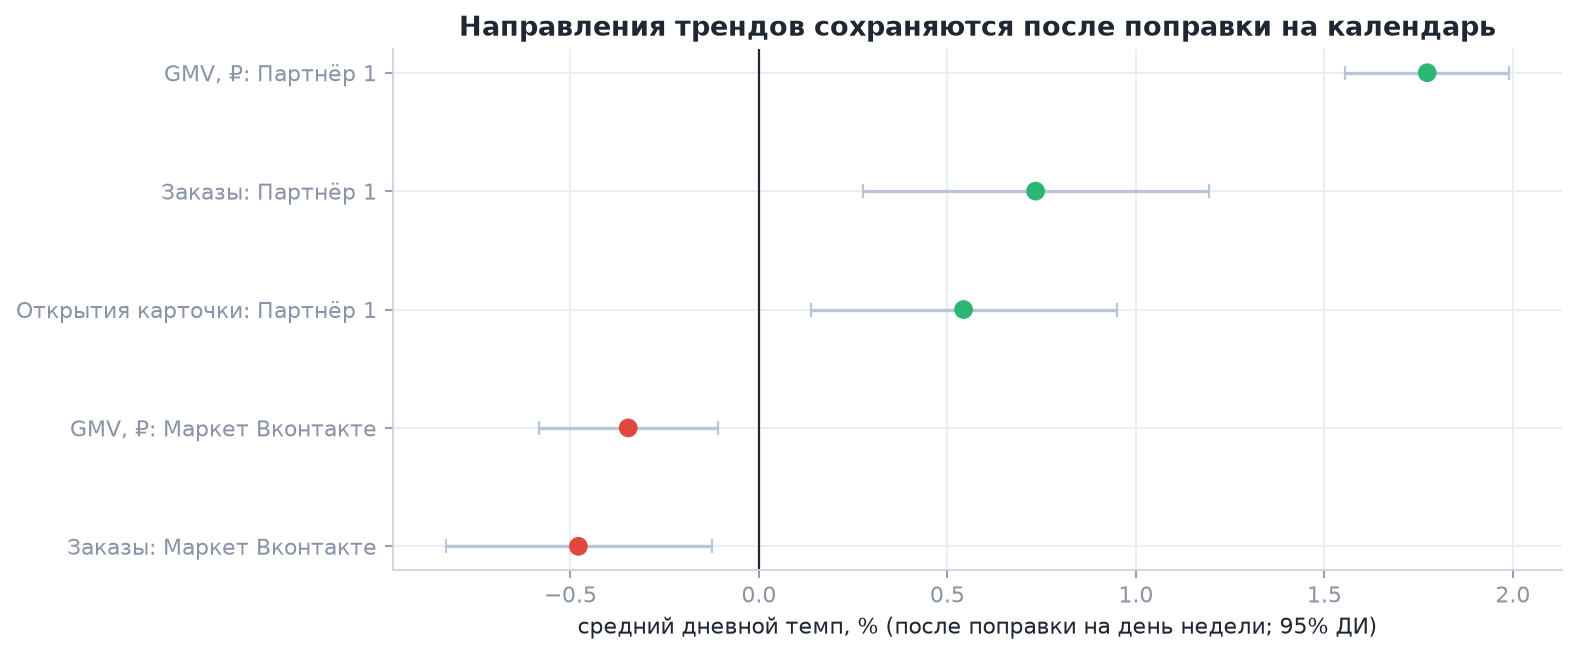
\includegraphics[width=\linewidth,height=0.70\textheight,keepaspectratio]{figures/05_trends_adjusted.png}
\caption*{Рис. 12. Направления трендов сохраняются после поправки на календарь}
\end{figure}

\textbf{Оговорка:} это один месяц и 30 наблюдений; сезонность и годовой цикл не оцениваются. Но направление устойчиво: \textbf{Маркет теряет заказы, Партнёр растёт} — ещё один аргумент, что проблема в механике Маркета, а не в рынке.\par

\subsection{Синтез: шесть выводов, которые держат стратегию}

\begingroup
\small
\setlength{\tabcolsep}{3pt}
\renewcommand{\arraystretch}{1.12}
\rowcolors{1}{white}{zebra}
\begin{longtable}{@{}>{\raggedright\arraybackslash}p{0.0306\linewidth}>{\raggedright\arraybackslash}p{0.2828\linewidth}>{\raggedright\arraybackslash}p{0.3439\linewidth}>{\raggedright\arraybackslash}p{0.3057\linewidth}@{}}
\rowcolor{blue}
\textcolor{white}{\textbf{№}} & \textcolor{white}{\textbf{Вывод}} & \textcolor{white}{\textbf{Доказательство}} & \textcolor{white}{\textbf{Что делать}} \\
\endfirsthead
\rowcolor{blue}
\textcolor{white}{\textbf{№}} & \textcolor{white}{\textbf{Вывод}} & \textcolor{white}{\textbf{Доказательство}} & \textcolor{white}{\textbf{Что делать}} \\
\endhead
\hline
1 & Узкое место — карточка → кнопка & 3,08\% vs 42,16\%; 106\% разрыва & кнопка «Купить» + чекаут по умолчанию \\
2 & Ассортимент — первый предиктор & OR 1,52; топ-1 ML; S5 39 SKU vs S4 9 & импорт каталога, расширение SKU \\
3 & Доставка необходима, но не достаточна & наивно ×3,2 → PSM +3,2 п.п., ДИ включает 0 & доставка «из коробки» + каталог + трафик \\
4 & Контент даёт охват, не конверсию & ×1,9 охват, ×0,54 ER, CTR 0,29\% & формат шопса, CTA, ссылка на карточку \\
5 & Реклама не доказала результат & 92,4\% без заказа; OR 1,02 & цель «заказ», атрибуция, ROAS \\
6 & Маркет — слой, не destination & 0,14\% DAU VK; 79,5\% браузинг; 28,6 млн поиска & каталог + чекаут + поиск + профиль \\
\hline
\end{longtable}
\endgroup
\vspace{4pt}

\clearpage

\section{Ответы на пять задач кейса}

\subsection{Задача 1: место ВКонтакте среди каналов}

\textbf{Короткий ответ:} ВКонтакте — не маркетплейс и не классифайд, а \textbf{канал социальной коммерции на стыке контента и сделки}. Его место — «там, где пользователь уже проводит время и доверяет автору/сообществу», а не «там, где он целенаправленно ищет товар».\par

\begingroup
\small
\setlength{\tabcolsep}{3pt}
\renewcommand{\arraystretch}{1.12}
\rowcolors{1}{white}{zebra}
\begin{longtable}{@{}>{\raggedright\arraybackslash}p{0.2165\linewidth}>{\raggedright\arraybackslash}p{0.2222\linewidth}>{\raggedright\arraybackslash}p{0.2621\linewidth}>{\raggedright\arraybackslash}p{0.2621\linewidth}@{}}
\rowcolor{blue}
\textcolor{white}{\textbf{Канал}} & \textcolor{white}{\textbf{Сила}} & \textcolor{white}{\textbf{Слабость}} & \textcolor{white}{\textbf{Место ВКонтакте}} \\
\endfirsthead
\rowcolor{blue}
\textcolor{white}{\textbf{Канал}} & \textcolor{white}{\textbf{Сила}} & \textcolor{white}{\textbf{Слабость}} & \textcolor{white}{\textbf{Место ВКонтакте}} \\
\endhead
\hline
Маркетплейсы (WB, Ozon, Яндекс Маркет) & трафик, логистика, доверие, ассортимент & высокая конкуренция, комиссии, слабый бренд продавца & не конкурировать лоб в лоб; быть витриной бренда и источником трафика \\
Классифайды (Авито) & локальный спрос, сделки & нет контента и бренда & партнёрство для локальных товаров \\
Собственный сайт & контроль, бренд, маржа & нет трафика, дорого привлекать & ВКонтакте приводит трафик и закрывает сделку \\
Мессенджеры & общение, каталог & нет витрины и контента & ВКонтакте даёт витрину + контент + оплату \\
Соцсети/контент & внимание, доверие, вдохновение & слабая сделка & \textbf{домашняя территория ВКонтакте} \\
\hline
\end{longtable}
\endgroup
\vspace{4pt}

\noindent\textbf{Уникальное предложение (черновик для слайда):}\par\vspace{4pt}

\begin{quote}
\noindent\colorbox{soft}{\parbox{\dimexpr\linewidth-2\fboxsep}{
\raggedright \textbf{ВКонтакте продаёт там, где аудитория уже живёт: контент приводит, сообщество вызывает доверие, карточка закрывает сделку, а Маркет даёт инфраструктуру — каталог, чекаут, доставку, оплату, поиск и профиль покупателя. Бизнесу не нужен свой сайт и своя логистика, чтобы получить первую продажу.}
}}
\end{quote}
\vspace{2pt}

\textbf{Что проверить дополнительно:} TikTok Shop (контент + affiliate + checkout), Instagram/Facebook Shops (каталог + checkout), Pinterest (inspiration → catalog), WhatsApp Business (catalog + chat), Avito (local commerce). В этом отчёте внешние бенчмарки не оцифрованы — это следующий шаг (см. раздел 11).\par

\subsection{Задача 2: целевые бизнесы и барьеры}

\textbf{Короткий ответ:} целевые — \textbf{S4 (2 922), S2 (2 096), S3 (320)}, с ростом у \textbf{S5/S6 (719)}. S0/S1 (3 697) — вне фокуса первого года.\par

\begingroup
\footnotesize
\setlength{\tabcolsep}{3pt}
\renewcommand{\arraystretch}{1.12}
\rowcolors{1}{white}{zebra}
\begin{longtable}{@{}>{\raggedright\arraybackslash}p{0.0401\linewidth}>{\raggedright\arraybackslash}p{0.2346\linewidth}>{\raggedright\arraybackslash}p{0.1602\linewidth}>{\raggedright\arraybackslash}p{0.1888\linewidth}>{\raggedright\arraybackslash}p{0.2632\linewidth}>{\raggedright\arraybackslash}p{0.0515\linewidth}@{}}
\rowcolor{blue}
\textcolor{white}{\textbf{Сегмент}} & \textcolor{white}{\textbf{Что нужно}} & \textcolor{white}{\textbf{Чего хочет}} & \textcolor{white}{\textbf{Барьер}} & \textcolor{white}{\textbf{Как помочь}} & \textcolor{white}{\textbf{Приоритет}} \\
\endfirsthead
\rowcolor{blue}
\textcolor{white}{\textbf{Сегмент}} & \textcolor{white}{\textbf{Что нужно}} & \textcolor{white}{\textbf{Чего хочет}} & \textcolor{white}{\textbf{Барьер}} & \textcolor{white}{\textbf{Как помочь}} & \textcolor{white}{\textbf{Приоритет}} \\
\endhead
\hline
S4 & доставка, оплата, расширение ассортимента & заказы без сайта и логистики & исполнение заказа, мало SKU & доставка/оплата «из коробки», импорт, обучение & \textbf{1} \\
S2 & каталог & попробовать продажи & нечего продавать & импорт Ozon/CSV/фото, карточка из фото & \textbf{2} \\
S3 & чекаут & получать заявки & сделка в сообщениях & чекаут по умолчанию & \textbf{3} \\
S5/S6 & трафик, повторные, оплата & масштаб & мало трафика, низкий CTR контента & шопсы, реклама на заказ, рефералка & \textbf{4} \\
S0/S1 & заявки, переписка & услуги & нет товара & вне фокуса кейса & — \\
\hline
\end{longtable}
\endgroup
\vspace{4pt}

\noindent\textbf{Приоритизация по эффекту (базовый сценарий):}\par\vspace{4pt}

\begingroup
\small
\setlength{\tabcolsep}{3pt}
\renewcommand{\arraystretch}{1.12}
\rowcolors{1}{white}{zebra}
\begin{longtable}{@{}>{\raggedright\arraybackslash}p{0.1626\linewidth}>{\raggedright\arraybackslash}p{0.5806\linewidth}>{\raggedright\arraybackslash}p{0.2322\linewidth}@{}}
\rowcolor{blue}
\textcolor{white}{\textbf{Сегмент}} & \textcolor{white}{\textbf{Новых продающих в выборке}} & \textcolor{white}{\textbf{Доля новых}} \\
\endfirsthead
\rowcolor{blue}
\textcolor{white}{\textbf{Сегмент}} & \textcolor{white}{\textbf{Новых продающих в выборке}} & \textcolor{white}{\textbf{Доля новых}} \\
\endhead
\hline
S4 & 46,8 & 63\% \\
S2 & 22,2 & 30\% \\
S3 & 5,0 & 7\% \\
\textbf{Итого} & \textbf{74,0} & \textbf{100\%} \\
\hline
\end{longtable}
\endgroup
\vspace{4pt}

\begin{figure}[htbp]
\centering
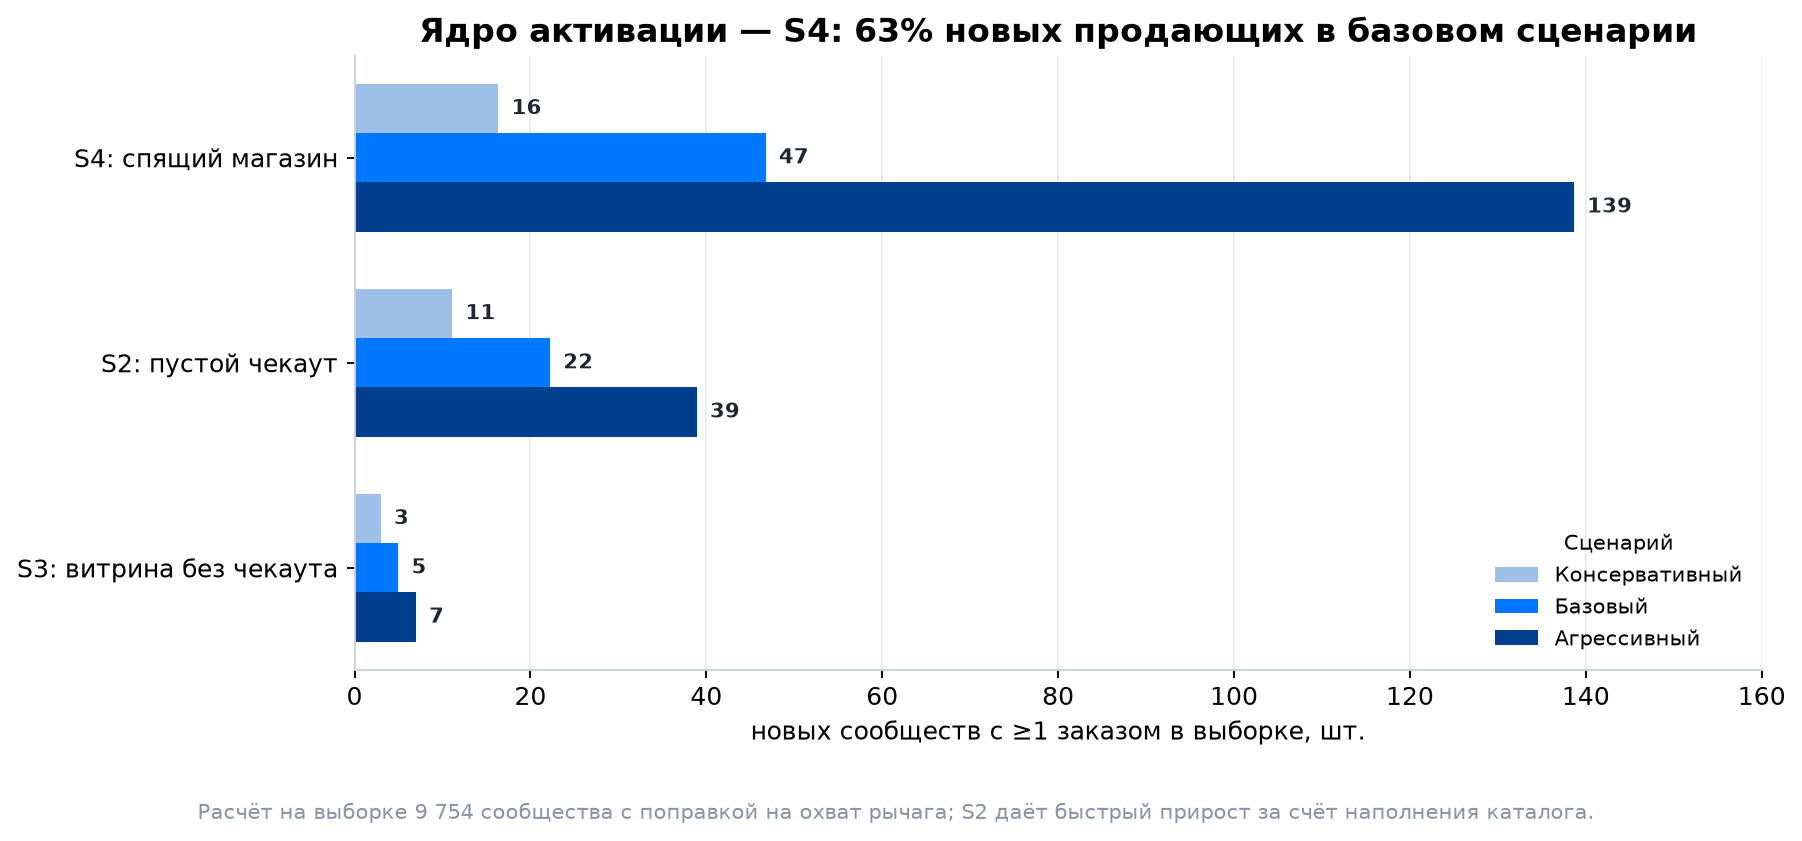
\includegraphics[width=\linewidth,height=0.70\textheight,keepaspectratio]{figures/report_priority.png}
\caption*{Рис. 13. Ядро активации — S4: 63\% новых продающих в базовом сценарии}
\end{figure}

\noindent\textbf{Барьеры, которые нельзя решить только продуктом:}\par\vspace{4pt}

\begin{itemize}[leftmargin=1.35em,itemsep=2pt,topsep=3pt,parsep=0pt]
\item \textbf{Доверие и привычка:} бизнес не верит, что ВКонтакте — канал продаж, а не «соцсеть для общения».
\item \textbf{Экономика:} комиссия + реклама + логистика должны оставлять маржу; для микро-СМБ это чувствительно.
\item \textbf{Компетенция:} нет контента, нет фото, нет понимания, что такое карточка и CTA.
\item \textbf{Атрибуция:} 98,8\% заказов не оплачены внутри VK; бизнес не видит полной картины.
\end{itemize}

\subsection{Задача 3: уникальное предложение и инструменты}

\textbf{Позиционирование:} «ВКонтакте — социальная витрина, которая доводит до сделки». Не «ещё один маркетплейс», а \textbf{слой продаж поверх сообщества и контента}.\par

\noindent\textbf{Пять рычагов:}\par\vspace{4pt}

\begingroup
\footnotesize
\setlength{\tabcolsep}{3pt}
\renewcommand{\arraystretch}{1.12}
\rowcolors{1}{white}{zebra}
\begin{longtable}{@{}>{\raggedright\arraybackslash}p{0.1188\linewidth}>{\raggedright\arraybackslash}p{0.1885\linewidth}>{\raggedright\arraybackslash}p{0.1885\linewidth}>{\raggedright\arraybackslash}p{0.1598\linewidth}>{\raggedright\arraybackslash}p{0.1885\linewidth}>{\raggedright\arraybackslash}p{0.0942\linewidth}@{}}
\rowcolor{blue}
\textcolor{white}{\textbf{Рычаг}} & \textcolor{white}{\textbf{Что делаем}} & \textcolor{white}{\textbf{Якорь из данных}} & \textcolor{white}{\textbf{Эффект для бизнеса}} & \textcolor{white}{\textbf{Эффект для VK}} & \textcolor{white}{\textbf{Как проверяем}} \\
\endfirsthead
\rowcolor{blue}
\textcolor{white}{\textbf{Рычаг}} & \textcolor{white}{\textbf{Что делаем}} & \textcolor{white}{\textbf{Якорь из данных}} & \textcolor{white}{\textbf{Эффект для бизнеса}} & \textcolor{white}{\textbf{Эффект для VK}} & \textcolor{white}{\textbf{Как проверяем}} \\
\endhead
\hline
\textbf{L1. Карточка = сделка} & кнопка «Купить», чекаут, статусы, оплата в 1 клик & 3,08\% vs 42,16\%; 106\% разрыва & сделка вместо переписки; выше конверсия & +1 п.п. кнопки = +134 тыс. заказов/мес и +507 млн ₽ GMV & E1: чекаут по умолчанию \\
\textbf{L2. Товарный контент и авторы} & шопсы в постах/клипах, рефералка, CTA & 3,1\% публикуют; CTR 0,29\%; 92,7\% открытий Партнёра — контент & новый трафик без своего продакшена & рост открытий и заказов; масштабирование модели Партнёра & E3: формат шопса \\
\textbf{L3. Релевантный ассортимент} & импорт каталога, чистка «мёртвого» трафика, локальные категории & OR SKU 1,52; 46,3\% открытий в категориях <0,1\% & быстрый старт, меньше пустых карточек & рост доли активного каталога и конверсии & E5: импорт каталога \\
\textbf{L4. Повторные покупки} & профиль покупателя, избранное, снижение цены, повторный заказ & 1,4 vs 1,7 заказа/покупателя; повторных 19\% vs 26,6\% & дешевле привлечения & +21\% заказов без нового трафика & профиль + уведомления \\
\textbf{L5. Активация сообществ} & доставка/оплата «из коробки», онбординг, триггеры & 94,8\% чекаутов не продают; PSM +3,2 п.п. & снятие барьера исполнения & рост числа продающих & E2: доставка \\
\hline
\end{longtable}
\endgroup
\vspace{4pt}

\noindent\textbf{Таблица двухсторонних эффектов (для слайда 6):}\par\vspace{4pt}

\begingroup
\footnotesize
\setlength{\tabcolsep}{3pt}
\renewcommand{\arraystretch}{1.12}
\rowcolors{1}{white}{zebra}
\begin{longtable}{@{}>{\raggedright\arraybackslash}p{0.1926\linewidth}>{\raggedright\arraybackslash}p{0.2287\linewidth}>{\raggedright\arraybackslash}p{0.2046\linewidth}>{\raggedright\arraybackslash}p{0.1504\linewidth}>{\raggedright\arraybackslash}p{0.1745\linewidth}@{}}
\rowcolor{blue}
\textcolor{white}{\textbf{Инструмент}} & \textcolor{white}{\textbf{Бизнес}} & \textcolor{white}{\textbf{ВКонтакте}} & \textcolor{white}{\textbf{Метрика}} & \textcolor{white}{\textbf{Риск}} \\
\endfirsthead
\rowcolor{blue}
\textcolor{white}{\textbf{Инструмент}} & \textcolor{white}{\textbf{Бизнес}} & \textcolor{white}{\textbf{ВКонтакте}} & \textcolor{white}{\textbf{Метрика}} & \textcolor{white}{\textbf{Риск}} \\
\endhead
\hline
Карточка с чекаутом по умолчанию & сделка вместо переписки & +1 п.п. = +134 тыс. заказов/мес & конверсия открытие→кнопка & продавец не исполнит заказ \\
Доставка и оплата «из коробки» & не нужно договариваться с перевозчиком & рост оплаченных заказов → комиссия & доля оплаченных & стоимость логистики, возвраты \\
Импорт каталога & каталог за минуты & 2 096 сообществ с пустым чекаутом & доля с активным каталогом & качество цен/наличия \\
Шопсы + рефералка & трафик без продакшена & рост открытий, заказов & CTR, заказ/1000 открытий & каннибализация рекламы \\
Реклама с целью «заказ» & видимый ROAS & удержание бюджета & ROAS, retention & краткосрочно CPC выше \\
Профиль покупателя & повторные дешевле & +21\% заказов & заказов на покупателя & нужна история заказов \\
Подписка Pro & предсказуемые расходы & диверсификация выручки & ARPA, churn & платят после первых продаж \\
\hline
\end{longtable}
\endgroup
\vspace{4pt}

\subsection{Задача 4: роль Маркета ВКонтакте}

\textbf{Короткий ответ:} \textbf{Маркет — слой товарной инфраструктуры и сделки, а не отдельный маркетплейс.} «Главную Маркета» как destination можно закрыть/переупаковать, но поиск, карточку, заказы и профиль покупателя нужно сохранить и встроить в сообщества.\par

\begingroup
\small
\setlength{\tabcolsep}{3pt}
\renewcommand{\arraystretch}{1.12}
\rowcolors{1}{white}{zebra}
\begin{longtable}{@{}>{\raggedright\arraybackslash}p{0.2437\linewidth}>{\raggedright\arraybackslash}p{0.2735\linewidth}>{\raggedright\arraybackslash}p{0.2140\linewidth}>{\raggedright\arraybackslash}p{0.2318\linewidth}@{}}
\rowcolor{blue}
\textcolor{white}{\textbf{Функция Маркета в целевой модели}} & \textcolor{white}{\textbf{Что делаем}} & \textcolor{white}{\textbf{Метрика}} & \textcolor{white}{\textbf{Почему важно}} \\
\endfirsthead
\rowcolor{blue}
\textcolor{white}{\textbf{Функция Маркета в целевой модели}} & \textcolor{white}{\textbf{Что делаем}} & \textcolor{white}{\textbf{Метрика}} & \textcolor{white}{\textbf{Почему важно}} \\
\endhead
\hline
Каталог и карточка (единый товарный слой) & карточка = сделка: цена, наличие, доставка, оплата, кнопка & открытие→нажатие (3,08\% → 8\%) & каждый +1 п.п. = +134 тыс. заказов/мес \\
Товарный поиск и рекомендации & интентный вход: 28,6 млн запросов/мес, 18,4\% с открытием & доля запросов с открытием/заказом & единственный канал с готовым намерением \\
Витрина внутри сообщества & магазин бренда/локального продавца, а не общая полка & заказы на сообщество, доля продающих & работает на региональный СМБ \\
Профиль покупателя и повторные & история, избранное, снижение цены, повторный заказ & заказов на покупателя 1,4 → 1,7 & +21\% заказов без нового трафика \\
Слой доверия и исполнения & доставка, оплата, возвраты, статусы, рейтинг & доля оплаченных (1,2\% → 50\%) & без этого нет комиссии \\
\hline
\end{longtable}
\endgroup
\vspace{4pt}

\noindent\textbf{Что не делать:}\par\vspace{4pt}

\begin{itemize}[leftmargin=1.35em,itemsep=2pt,topsep=3pt,parsep=0pt]
\item не строить собственную логистику и склад;
\item не конкурировать с WB/Ozon по ассортименту и цене;
\item не тащить весь трафик на «Главную Маркета»;
\item не обещать «×3 от доставки» — после PSM эффект +3 п.п. и незначим.
\end{itemize}

\subsection{Задача 5: целевой путь с развилками}

\textbf{Логика пути:} общий вход → развилка «есть ли товар?» → три трека (S2 / S3-S4 / S5-S6) → первая продажа → повторные → масштаб.\par

\begin{figure}[htbp]
\centering
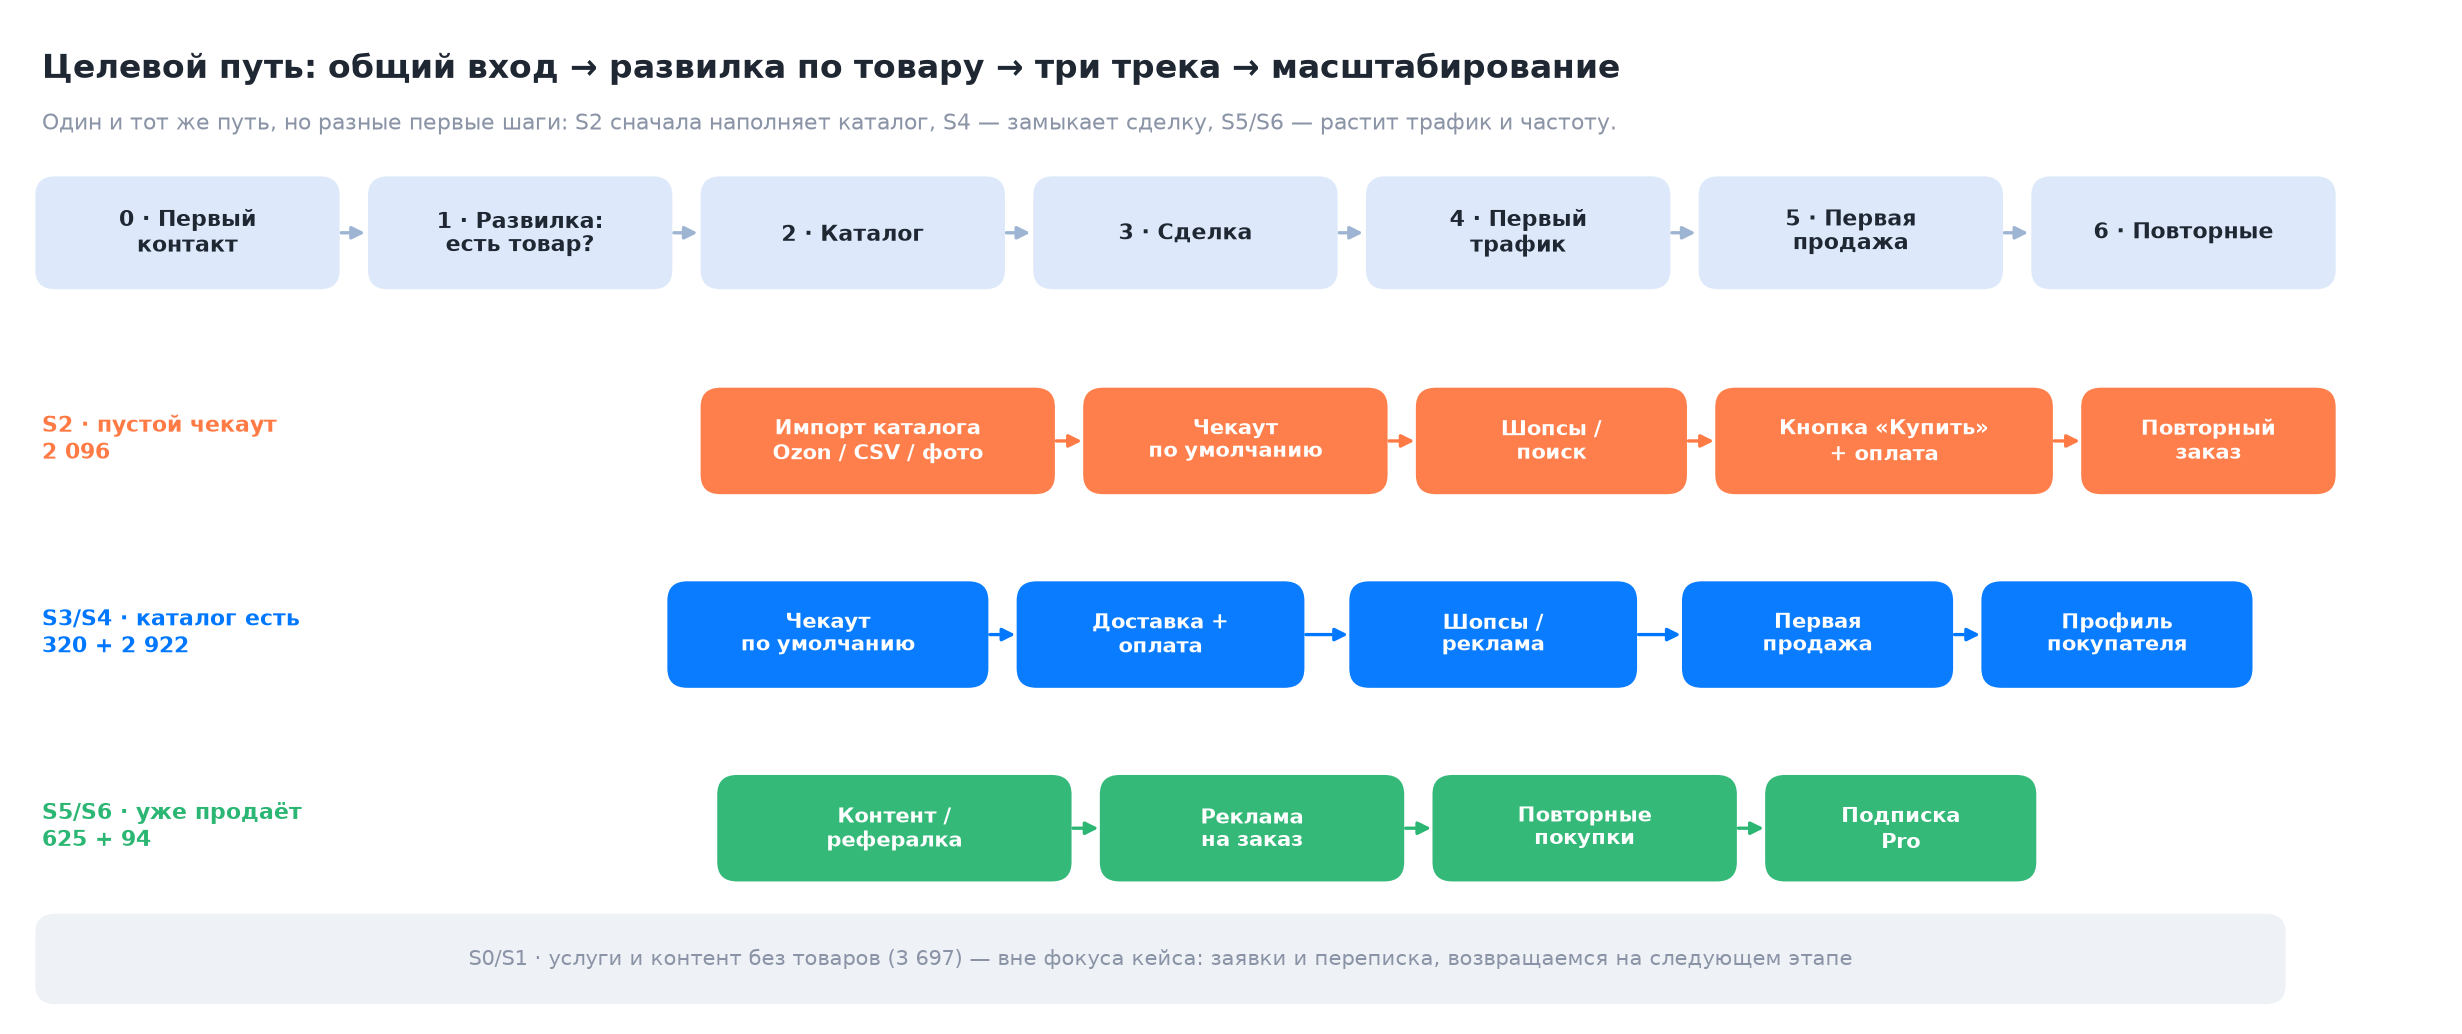
\includegraphics[width=\linewidth,height=0.70\textheight,keepaspectratio]{figures/report_tracks.png}
\caption*{Рис. 14. Целевой путь: общий вход, развилка по товару, три трека}
\end{figure}

\begingroup
\footnotesize
\setlength{\tabcolsep}{3pt}
\renewcommand{\arraystretch}{1.12}
\rowcolors{1}{white}{zebra}
\begin{longtable}{@{}>{\raggedright\arraybackslash}p{0.1255\linewidth}>{\raggedright\arraybackslash}p{0.1104\linewidth}>{\raggedright\arraybackslash}p{0.0602\linewidth}>{\raggedright\arraybackslash}p{0.2308\linewidth}>{\raggedright\arraybackslash}p{0.1807\linewidth}>{\raggedright\arraybackslash}p{0.2308\linewidth}@{}}
\rowcolor{blue}
\textcolor{white}{\textbf{Этап}} & \textcolor{white}{\textbf{Задача бизнеса}} & \textcolor{white}{\textbf{Сегменты}} & \textcolor{white}{\textbf{Инструменты VK}} & \textcolor{white}{\textbf{Метрика этапа}} & \textcolor{white}{\textbf{Развилка}} \\
\endfirsthead
\rowcolor{blue}
\textcolor{white}{\textbf{Этап}} & \textcolor{white}{\textbf{Задача бизнеса}} & \textcolor{white}{\textbf{Сегменты}} & \textcolor{white}{\textbf{Инструменты VK}} & \textcolor{white}{\textbf{Метрика этапа}} & \textcolor{white}{\textbf{Развилка}} \\
\endhead
\hline
0. Первый контакт & узнать о продажах в VK & все & сообщество с целью «Развивать бизнес», чек-лист & создано сообщество с инструментами & — \\
1. Развилка «есть товар?» & выбрать сценарий & все & опрос из 3 вопросов, автоопределение & доля прошедших маршрутизацию & услуги → трек «заявки» (вне фокуса) \\
2a. Нет каталога & наполнить каталог & S2 & импорт Ozon/CSV/фото→карточка & доля с активным каталогом & нет товара физически → предзаказ/хендмейд \\
2b. Есть каталог & включить сделку & S3/S4 & чекаут по умолчанию, шаблоны доставки & доля с чекаутом и доставкой & — \\
3. Настройка сделки & исполнение заказа & S3/S4/S5 & доставка «из коробки», оплата, статусы, возвраты & доля с полным стеком & самовывоз/локальная доставка → упрощённый стек \\
4. Первый трафик & привести посетителей & все товарные & шопсы, поиск, SEO карточки & открытия на сообщество; CTR & нет контента → реклама на карточку; есть авторы → рефералка \\
5. Первая продажа & момент истины & все товарные & кнопка, оплата в 1 клик, трекинг & доля с ≥1 заказом (3,1\% → 6–10\%) & нет заказа за 14 дней → триггерная помощь \\
6. Повторные & удержать покупателя & S5/S6 & профиль, избранное, снижение цены & заказов на покупателя 1,4 → 1,7 & — \\
7. Масштаб & рост и монетизация & S5/S6 & реклама на заказ, рефералка, Pro & GMV на продавца, ROAS, доля платящих & — \\
\hline
\end{longtable}
\endgroup
\vspace{4pt}

\noindent\textbf{Развилки по сегментам:}\par\vspace{4pt}

\begingroup
\small
\setlength{\tabcolsep}{3pt}
\renewcommand{\arraystretch}{1.12}
\rowcolors{1}{white}{zebra}
\begin{longtable}{@{}>{\raggedright\arraybackslash}p{0.0994\linewidth}>{\raggedright\arraybackslash}p{0.3057\linewidth}>{\raggedright\arraybackslash}p{0.3516\linewidth}>{\raggedright\arraybackslash}p{0.2064\linewidth}@{}}
\rowcolor{blue}
\textcolor{white}{\textbf{Сегмент}} & \textcolor{white}{\textbf{Последовательность}} & \textcolor{white}{\textbf{Почему так}} & \textcolor{white}{\textbf{Ключевой инструмент}} \\
\endfirsthead
\rowcolor{blue}
\textcolor{white}{\textbf{Сегмент}} & \textcolor{white}{\textbf{Последовательность}} & \textcolor{white}{\textbf{Почему так}} & \textcolor{white}{\textbf{Ключевой инструмент}} \\
\endhead
\hline
S2 (2 096) & каталог → сделка → контент & нечего продавать; сначала наполнение & импорт каталога \\
S3 (320) & чекаут → доставка → контент & сделка уходит в сообщения & чекаут по умолчанию \\
S4 (2 922) & доставка/оплата → контент → реклама & ассортимент мал, исполнение не настроено & пакет «логистика под ключ» \\
S5/S6 (719) & контент/рефералка → повторные → подписка & сделка работает, узкое место — трафик и частота & шопсы + реклама на карточку \\
S0/S1 (3 697) & заявки/сообщения & нет товара & вне фокуса \\
\hline
\end{longtable}
\endgroup
\vspace{4pt}

\clearpage

\section{Целевая концепция: «Маркет как слой»}

\subsection{Формулировка}

\begin{quote}
\noindent\colorbox{soft}{\parbox{\dimexpr\linewidth-2\fboxsep}{
\raggedright \textbf{Маркет ВКонтакте — это не место, куда приходят за товаром, а слой, который превращает контент и сообщество в сделку.} Он даёт бизнесу каталог, карточку, чекаут, доставку, оплату, поиск и профиль покупателя; ВКонтакте — трафик, доверие и контент. Маркет перестаёт быть «ещё одной витриной» и становится инфраструктурой социальной коммерции.
}}
\end{quote}
\vspace{2pt}

\subsection{Три горизонта}

\begingroup
\small
\setlength{\tabcolsep}{3pt}
\renewcommand{\arraystretch}{1.12}
\rowcolors{1}{white}{zebra}
\begin{longtable}{@{}>{\raggedright\arraybackslash}p{0.0808\linewidth}>{\raggedright\arraybackslash}p{0.2626\linewidth}>{\raggedright\arraybackslash}p{0.3098\linewidth}>{\raggedright\arraybackslash}p{0.3098\linewidth}@{}}
\rowcolor{blue}
\textcolor{white}{\textbf{Горизонт}} & \textcolor{white}{\textbf{Фокус}} & \textcolor{white}{\textbf{Что делаем}} & \textcolor{white}{\textbf{Ожидаемый результат}} \\
\endfirsthead
\rowcolor{blue}
\textcolor{white}{\textbf{Горизонт}} & \textcolor{white}{\textbf{Фокус}} & \textcolor{white}{\textbf{Что делаем}} & \textcolor{white}{\textbf{Ожидаемый результат}} \\
\endhead
\hline
0–90 дней & замкнуть сделку на существующем трафике & чекаут по умолчанию, кнопка «Купить», E1/E3, дашборд воронки & конверсия кнопки 3,1\% → 5\%; +130 тыс. заказов/мес \\
3–6 месяцев & исполнение и ассортимент & доставка/оплата «из коробки», импорт каталога, E2/E5, товарный поиск & оплаченные заказы 1,2\% → 25\%; продающие 3,1\% → 3,8–4,9\% \\
6–12 месяцев & масштаб и монетизация & шопсы + рефералка, реклама на заказ, профиль, Pro, комиссия & кнопка 8\%; 1,7 млн заказов/мес; 143 млн ₽/мес \\
\hline
\end{longtable}
\endgroup
\vspace{4pt}

\subsection{Что меняется для бизнеса}

\begingroup
\small
\setlength{\tabcolsep}{3pt}
\renewcommand{\arraystretch}{1.12}
\rowcolors{1}{white}{zebra}
\begin{longtable}{@{}>{\raggedright\arraybackslash}p{0.4100\linewidth}>{\raggedright\arraybackslash}p{0.5777\linewidth}@{}}
\rowcolor{blue}
\textcolor{white}{\textbf{Было}} & \textcolor{white}{\textbf{Стало}} \\
\endfirsthead
\rowcolor{blue}
\textcolor{white}{\textbf{Было}} & \textcolor{white}{\textbf{Стало}} \\
\endhead
\hline
сообщество + переписка & сообщество + карточка + сделка \\
свой сайт и логистика & витрина и доставка «из коробки» \\
непонятный охват & видимые заказы и ROAS \\
разовые продажи & повторные покупки и профиль \\
«ещё одна соцсеть» & канал продаж с экономикой \\
\hline
\end{longtable}
\endgroup
\vspace{4pt}

\subsection{Что меняется для ВКонтакте}

\begingroup
\small
\setlength{\tabcolsep}{3pt}
\renewcommand{\arraystretch}{1.12}
\rowcolors{1}{white}{zebra}
\begin{longtable}{@{}>{\raggedright\arraybackslash}p{0.4669\linewidth}>{\raggedright\arraybackslash}p{0.5208\linewidth}@{}}
\rowcolor{blue}
\textcolor{white}{\textbf{Было}} & \textcolor{white}{\textbf{Стало}} \\
\endfirsthead
\rowcolor{blue}
\textcolor{white}{\textbf{Было}} & \textcolor{white}{\textbf{Стало}} \\
\endhead
\hline
реклама как основной доход & реклама + комиссия + подписка \\
оптимизация на охват & оптимизация на заказ \\
Маркет как витрина & Маркет как инфраструктура \\
3,1\% продающих & 3,8–4,9\% в базовом сценарии \\
413,7 тыс. заказов/мес & 1,70 млн заказов/мес \\
\hline
\end{longtable}
\endgroup
\vspace{4pt}

\clearpage

\section{Сценарии, монетизация и KPI}

\subsection{Допущения модели}

Модель считает \textbf{не от выборки}, а от платформенных метрик сентября 2026:\par

\begin{itemize}[leftmargin=1.35em,itemsep=2pt,topsep=3pt,parsep=0pt]
\item открытия карточки: 193,5 млн/мес;
\item нажатия кнопки: 3,08\% (база);
\item нажатие → заказ: 6,93\% (база);
\item заказы: 413,7 тыс./мес;
\item AOV: 3 781 ₽ (база);
\item оплаченная доля: 1,19\% (факт);
\item заказов на покупателя: 1,40.
\end{itemize}

Сценарии меняют \textbf{явные параметры}:\par

\begingroup
\small
\setlength{\tabcolsep}{3pt}
\renewcommand{\arraystretch}{1.12}
\rowcolors{1}{white}{zebra}
\begin{longtable}{@{}>{\raggedright\arraybackslash}p{0.4224\linewidth}>{\raggedright\arraybackslash}p{0.2365\linewidth}>{\raggedright\arraybackslash}p{0.1183\linewidth}>{\raggedright\arraybackslash}p{0.1858\linewidth}@{}}
\rowcolor{blue}
\textcolor{white}{\textbf{Параметр}} & \textcolor{white}{\textbf{Консервативный}} & \textcolor{white}{\textbf{Базовый}} & \textcolor{white}{\textbf{Агрессивный}} \\
\endfirsthead
\rowcolor{blue}
\textcolor{white}{\textbf{Параметр}} & \textcolor{white}{\textbf{Консервативный}} & \textcolor{white}{\textbf{Базовый}} & \textcolor{white}{\textbf{Агрессивный}} \\
\endhead
\hline
Конверсия открытие→кнопка & 5,0\% & 8,0\% & 15,0\% \\
Конверсия кнопка→заказ & 8,0\% & 10,0\% & 12,0\% \\
Рост открытий & 0\% & +10\% & +25\% \\
AOV, ₽ & 3 600 & 3 300 & 2 900 \\
Заказов на покупателя & 1,45 & 1,55 & 1,70 \\
Оплаченная доля & 25\% & 50\% & 70\% \\
Take rate & 3\% & 5\% & 7\% \\
\hline
\end{longtable}
\endgroup
\vspace{4pt}

\textbf{Проверка на реализуемость:} даже агрессивные 15\% кнопки — это лишь \textbf{36\% от уровня Партнёра (42,16\%)}, который уже работает на том же трафике ВКонтакте. Мы не предполагаем чуда, а частично закрываем доказанный разрыв.\par

\subsection{Платформенный эффект}

\begingroup
\footnotesize
\setlength{\tabcolsep}{3pt}
\renewcommand{\arraystretch}{1.12}
\rowcolors{1}{white}{zebra}
\begin{longtable}{@{}>{\raggedright\arraybackslash}p{0.1493\linewidth}>{\raggedright\arraybackslash}p{0.1066\linewidth}>{\raggedright\arraybackslash}p{0.1493\linewidth}>{\raggedright\arraybackslash}p{0.1600\linewidth}>{\raggedright\arraybackslash}p{0.1493\linewidth}>{\raggedright\arraybackslash}p{0.2239\linewidth}@{}}
\rowcolor{blue}
\textcolor{white}{\textbf{Сценарий}} & \textcolor{white}{\textbf{Заказы/мес}} & \textcolor{white}{\textbf{Прирост к базе}} & \textcolor{white}{\textbf{GMV/мес, млрд ₽}} & \textcolor{white}{\textbf{Покупатели/мес}} & \textcolor{white}{\textbf{Оплаченные заказы/мес}} \\
\endfirsthead
\rowcolor{blue}
\textcolor{white}{\textbf{Сценарий}} & \textcolor{white}{\textbf{Заказы/мес}} & \textcolor{white}{\textbf{Прирост к базе}} & \textcolor{white}{\textbf{GMV/мес, млрд ₽}} & \textcolor{white}{\textbf{Покупатели/мес}} & \textcolor{white}{\textbf{Оплаченные заказы/мес}} \\
\endhead
\hline
База & 413 740 & — & 1,56 & 296 148 & 4 903 \\
Консервативный & 774 050 & +87\% & 2,79 & 533 828 & 193 512 \\
Базовый & 1 702 910 & +312\% & 5,62 & 1 098 651 & 851 455 \\
Агрессивный & 4 354 030 & +952\% & 12,63 & 2 561 194 & 3 047 821 \\
\hline
\end{longtable}
\endgroup
\vspace{4pt}

\begin{figure}[htbp]
\centering
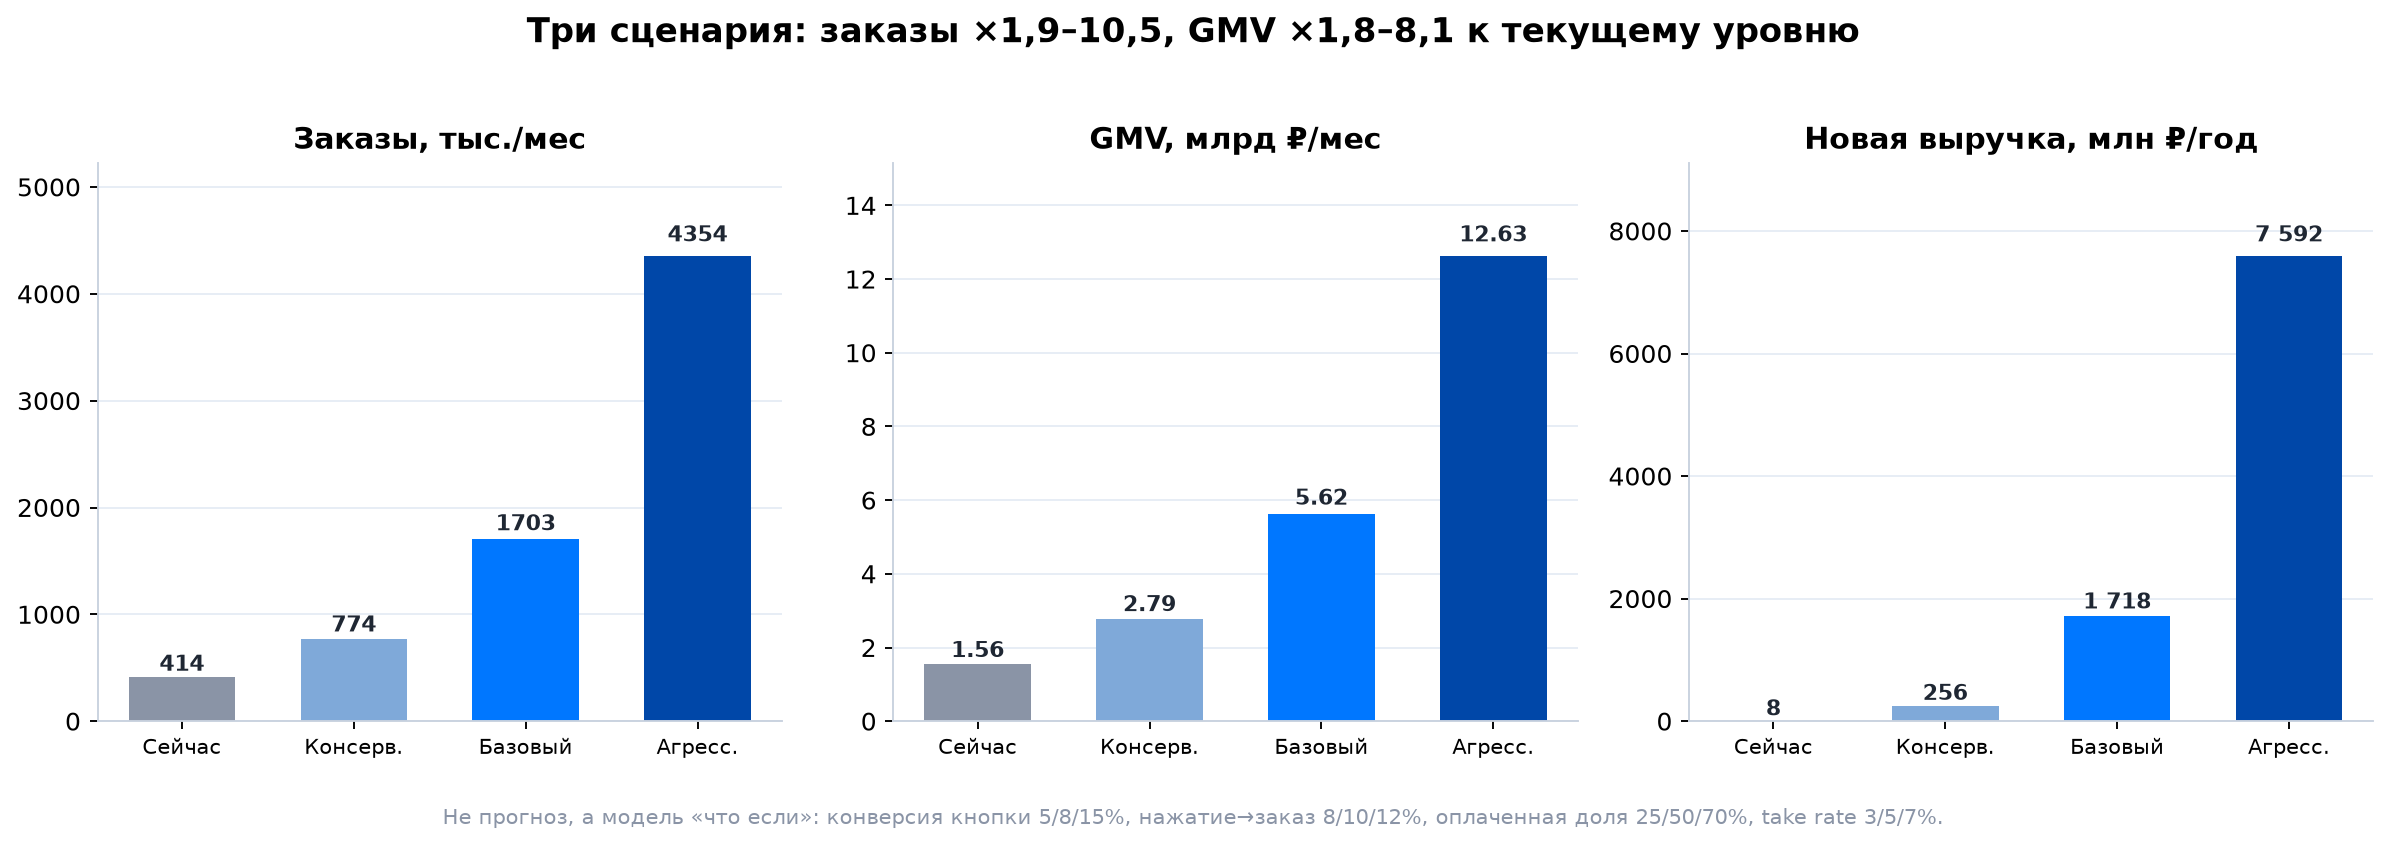
\includegraphics[width=\linewidth,height=0.70\textheight,keepaspectratio]{figures/report_scenarios.png}
\caption*{Рис. 15. Три сценария: заказы, GMV и новая выручка}
\end{figure}

\subsection{Монетизация}

\begingroup
\scriptsize
\setlength{\tabcolsep}{3pt}
\renewcommand{\arraystretch}{1.12}
\rowcolors{1}{white}{zebra}
\begin{longtable}{@{}>{\raggedright\arraybackslash}p{0.1080\linewidth}>{\raggedright\arraybackslash}p{0.2007\linewidth}>{\raggedright\arraybackslash}p{0.0695\linewidth}>{\raggedright\arraybackslash}p{0.1466\linewidth}>{\raggedright\arraybackslash}p{0.1466\linewidth}>{\raggedright\arraybackslash}p{0.1235\linewidth}>{\raggedright\arraybackslash}p{0.1312\linewidth}@{}}
\rowcolor{blue}
\textcolor{white}{\textbf{Сценарий}} & \textcolor{white}{\textbf{Оплаченный GMV, млрд ₽/мес}} & \textcolor{white}{\textbf{Take rate}} & \textcolor{white}{\textbf{Комиссия, млн ₽/мес}} & \textcolor{white}{\textbf{Подписка, млн ₽/мес}} & \textcolor{white}{\textbf{Итого, млн ₽/мес}} & \textcolor{white}{\textbf{Итого, млрд ₽/год}} \\
\endfirsthead
\rowcolor{blue}
\textcolor{white}{\textbf{Сценарий}} & \textcolor{white}{\textbf{Оплаченный GMV, млрд ₽/мес}} & \textcolor{white}{\textbf{Take rate}} & \textcolor{white}{\textbf{Комиссия, млн ₽/мес}} & \textcolor{white}{\textbf{Подписка, млн ₽/мес}} & \textcolor{white}{\textbf{Итого, млн ₽/мес}} & \textcolor{white}{\textbf{Итого, млрд ₽/год}} \\
\endhead
\hline
Консервативный & 0,70 & 3\% & 20,9 & 0,4 & 21,3 & 0,26 \\
Базовый & 2,81 & 5\% & 140,5 & 2,7 & \textbf{143,2} & \textbf{1,72} \\
Агрессивный & 8,84 & 7\% & 618,7 & 14,0 & 632,7 & 7,59 \\
\hline
\end{longtable}
\endgroup
\vspace{4pt}

\noindent\textbf{Важно:}\par\vspace{4pt}

\begin{itemize}[leftmargin=1.35em,itemsep=2pt,topsep=3pt,parsep=0pt]
\item комиссия берётся \textbf{только с оплаченного GMV}, поэтому так важна доля оплаты (1,2\% → 50\%);
\item подписка — не «доступ к продажам», а \textbf{Pro-инструменты} (аналитика, автоответы, статусы, приоритет);
\item рост рекламной выручки (+10/25/50\%) в таблицу \textbf{не включён} — это отдельный upside, его нельзя складывать с комиссией без проверки каннибализации;
\item текущая база комиссии и подписки — около \textbf{0,7 млн ₽/мес}, то есть базовый сценарий — это не «+143 млн к 143», а рост с почти нуля.
\end{itemize}

\subsection{Чувствительность}

\begingroup
\small
\setlength{\tabcolsep}{3pt}
\renewcommand{\arraystretch}{1.12}
\rowcolors{1}{white}{zebra}
\begin{longtable}{@{}>{\raggedright\arraybackslash}p{0.1778\linewidth}>{\raggedright\arraybackslash}p{0.1926\linewidth}>{\raggedright\arraybackslash}p{0.1926\linewidth}>{\raggedright\arraybackslash}p{0.4000\linewidth}@{}}
\rowcolor{blue}
\textcolor{white}{\textbf{Параметр}} & \textcolor{white}{\textbf{−50\%}} & \textcolor{white}{\textbf{+50\%}} & \textcolor{white}{\textbf{Вывод}} \\
\endfirsthead
\rowcolor{blue}
\textcolor{white}{\textbf{Параметр}} & \textcolor{white}{\textbf{−50\%}} & \textcolor{white}{\textbf{+50\%}} & \textcolor{white}{\textbf{Вывод}} \\
\endhead
\hline
click\_rate & −50\% заказов & +50\% заказов & главный рычаг \\
click2order & −50\% заказов & +50\% заказов & главный рычаг \\
opens\_growth & −4,5\% заказов & +4,5\% заказов & трафик вторичен \\
aov & — & — & влияет на GMV, не на заказы \\
paid\_share & — & — & влияет на комиссию \\
take\_rate & — & — & влияет на комиссию \\
\hline
\end{longtable}
\endgroup
\vspace{4pt}

\begin{figure}[htbp]
\centering
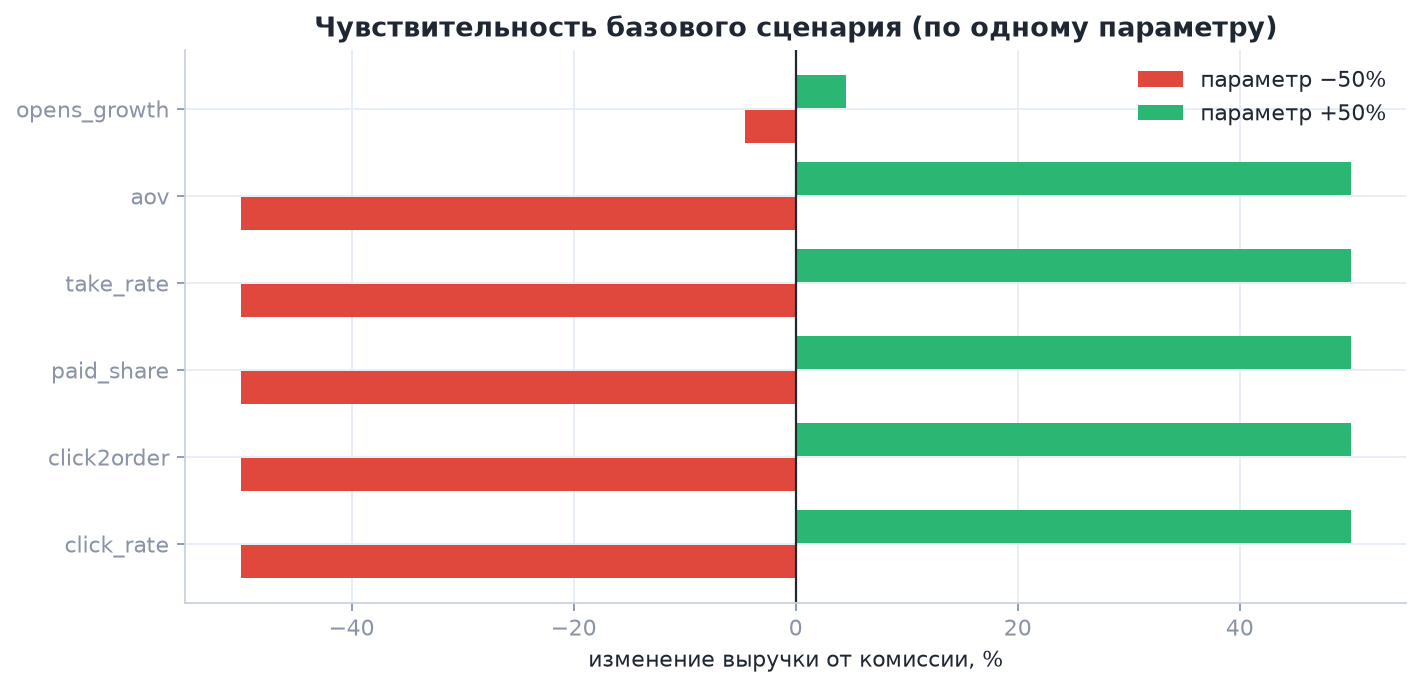
\includegraphics[width=\linewidth,height=0.70\textheight,keepaspectratio]{figures/04_sensitivity.png}
\caption*{Рис. 16. Чувствительность базового сценария}
\end{figure}

\textbf{Вывод:} спор о трафике менее важен, чем спор о конверсии кнопки и оплате. Именно поэтому E1/E2 — приоритетные эксперименты.\par

\subsection{KPI-дерево}

\begingroup
\small
\setlength{\tabcolsep}{3pt}
\renewcommand{\arraystretch}{1.12}
\rowcolors{1}{white}{zebra}
\begin{longtable}{@{}>{\raggedright\arraybackslash}p{0.1246\linewidth}>{\raggedright\arraybackslash}p{0.4305\linewidth}>{\raggedright\arraybackslash}p{0.1586\linewidth}>{\raggedright\arraybackslash}p{0.2493\linewidth}@{}}
\rowcolor{blue}
\textcolor{white}{\textbf{Уровень}} & \textcolor{white}{\textbf{Метрика}} & \textcolor{white}{\textbf{Сейчас}} & \textcolor{white}{\textbf{Цель (базовый, 12 мес)}} \\
\endfirsthead
\rowcolor{blue}
\textcolor{white}{\textbf{Уровень}} & \textcolor{white}{\textbf{Метрика}} & \textcolor{white}{\textbf{Сейчас}} & \textcolor{white}{\textbf{Цель (базовый, 12 мес)}} \\
\endhead
\hline
North Star & доля сообществ с ≥1 заказом за 30 дней & 3,1\% & 3,4–4,9\% (база 3,8\%) \\
Ведущий 1 & доля с активным каталогом & 40,6\% & 44,9\% \\
Ведущий 2 & доля с доставкой / оплатой & 9,4\% / 2,6\% & 24,4\% / 15\% \\
Ведущий 3 & доля публикующих товарный контент & 3,1\% & 15\% (вне модели) \\
Воронка 1 & открытие→кнопка & 3,08\% & 8\% \\
Воронка 2 & доля оплаченных заказов & 1,19\% & 50\% \\
Воронка 3 & CTR товарного контента & 0,29\% & 1,0\% (вне модели) \\
Результат 1 & заказы/мес & 413,7 тыс. & 1,70 млн \\
Результат 2 & GMV/мес & 1,56 млрд ₽ & 5,62 млрд ₽ \\
Результат 3 & заказов на покупателя & 1,4 & 1,7 \\
Монетизация & комиссия + подписка & ≈0,7 млн ₽/мес & 143 млн ₽/мес \\
Здоровье & доля рекламодателей с заказом & 7,6\% & 40\% \\
\hline
\end{longtable}
\endgroup
\vspace{4pt}

\clearpage

\section{План проверки: эксперименты, дорожная карта, риски}

\subsection{Пять экспериментов}

\begingroup
\footnotesize
\setlength{\tabcolsep}{3pt}
\renewcommand{\arraystretch}{1.12}
\rowcolors{1}{white}{zebra}
\begin{longtable}{@{}>{\raggedright\arraybackslash}p{0.0239\linewidth}>{\raggedright\arraybackslash}p{0.1793\linewidth}>{\raggedright\arraybackslash}p{0.1853\linewidth}>{\raggedright\arraybackslash}p{0.0897\linewidth}>{\raggedright\arraybackslash}p{0.2630\linewidth}>{\raggedright\arraybackslash}p{0.1972\linewidth}@{}}
\rowcolor{blue}
\textcolor{white}{\textbf{\#}} & \textcolor{white}{\textbf{Эксперимент}} & \textcolor{white}{\textbf{Аудитория}} & \textcolor{white}{\textbf{Дизайн}} & \textcolor{white}{\textbf{Метрики}} & \textcolor{white}{\textbf{Мощность}} \\
\endfirsthead
\rowcolor{blue}
\textcolor{white}{\textbf{\#}} & \textcolor{white}{\textbf{Эксперимент}} & \textcolor{white}{\textbf{Аудитория}} & \textcolor{white}{\textbf{Дизайн}} & \textcolor{white}{\textbf{Метрики}} & \textcolor{white}{\textbf{Мощность}} \\
\endhead
\hline
E1 & Чекаут по умолчанию & S3+S4, 3 242 & 50/50, 4 недели & доля с ≥1 заказом; заказы/сообщество & MDE +2 п.п. при α=0,05, power=0,8 \\
E2 & Доставка «из коробки» & S4, 2 922 & 50/50, 6 недель & активация, заказы, отмены & ATT +3,2 п.п. → ≈2 500/группа \\
E3 & Формат шопса (цена/скидка/CTA) & сообщества с товарным контентом & A/B/C, 3 недели & CTR просмотр→карточка; заказ/1000 открытий & базовый CTR 0,29\% → +0,1 п.п. \\
E4 & Реклама с целью «заказ» & 542 плательщика & 50/50, 4 недели & ROAS, retention бюджета & GMV через чекаут — нижняя оценка \\
E5 & Импорт каталога & S2, 2 096 & 50/50, 4 недели & доля с активным каталогом; время до карточки & высокая база эффекта \\
\hline
\end{longtable}
\endgroup
\vspace{4pt}

\subsection{Дорожная карта}

\begingroup
\small
\setlength{\tabcolsep}{3pt}
\renewcommand{\arraystretch}{1.12}
\rowcolors{1}{white}{zebra}
\begin{longtable}{@{}>{\raggedright\arraybackslash}p{0.0903\linewidth}>{\raggedright\arraybackslash}p{0.1806\linewidth}>{\raggedright\arraybackslash}p{0.3461\linewidth}>{\raggedright\arraybackslash}p{0.3461\linewidth}@{}}
\rowcolor{blue}
\textcolor{white}{\textbf{Горизонт}} & \textcolor{white}{\textbf{Фокус}} & \textcolor{white}{\textbf{Что делаем}} & \textcolor{white}{\textbf{Результат}} \\
\endfirsthead
\rowcolor{blue}
\textcolor{white}{\textbf{Горизонт}} & \textcolor{white}{\textbf{Фокус}} & \textcolor{white}{\textbf{Что делаем}} & \textcolor{white}{\textbf{Результат}} \\
\endhead
\hline
0–90 дней & замкнуть сделку & чекаут по умолчанию, кнопка, E1/E3, дашборд & кнопка 3,1\% → 5\%; +130 тыс. заказов/мес \\
3–6 месяцев & исполнение и ассортимент & доставка/оплата, импорт, E2/E5, поиск & оплаченные 1,2\% → 25\%; продающие 3,1\% → 3,8–4,9\% \\
6–12 месяцев & масштаб и монетизация & шопсы, рефералка, реклама на заказ, профиль, Pro, комиссия & кнопка 8\%; 1,7 млн заказов/мес; 143 млн ₽/мес \\
\hline
\end{longtable}
\endgroup
\vspace{4pt}

\subsection{Риски}

\begingroup
\small
\setlength{\tabcolsep}{3pt}
\renewcommand{\arraystretch}{1.12}
\rowcolors{1}{white}{zebra}
\begin{longtable}{@{}>{\raggedright\arraybackslash}p{0.2913\linewidth}>{\raggedright\arraybackslash}p{0.0890\linewidth}>{\raggedright\arraybackslash}p{0.2104\linewidth}>{\raggedright\arraybackslash}p{0.3723\linewidth}@{}}
\rowcolor{blue}
\textcolor{white}{\textbf{Риск}} & \textcolor{white}{\textbf{Вероятность}} & \textcolor{white}{\textbf{Проявление}} & \textcolor{white}{\textbf{Как снимаем}} \\
\endfirsthead
\rowcolor{blue}
\textcolor{white}{\textbf{Риск}} & \textcolor{white}{\textbf{Вероятность}} & \textcolor{white}{\textbf{Проявление}} & \textcolor{white}{\textbf{Как снимаем}} \\
\endhead
\hline
Продавец не может исполнить заказ & высокая & отмены, негатив & чекаут только с доставкой/самовывозом; пилот на 2 регионах \\
Каннибализация рекламной выручки & средняя & комиссия вместо рекламы & суммарный take rate; комиссия только с оплаченного GMV \\
Данные не позволяют измерить эффект & высокая & 98,8\% заказов не оплачены & атрибуция и статусы; единый ID сделки; сквозная аналитика \\
Партнёр уводит трафик мимо VK & средняя & 106,9 млн прямых переходов & чекаут внутри VK для части ассортимента; ценность — новый трафик \\
Эффекты переоценены (self-selection) & высокая & наивно ×3,2 вместо ×1,2 & все обещания через A/B; ДИ в презентации \\
Синтетичность данных & высокая & часть цифр искажена & структурные выводы + чувствительность + вопросы экспертам \\
\hline
\end{longtable}
\endgroup
\vspace{4pt}

\subsection{Что нельзя утверждать}

\begingroup
\small
\setlength{\tabcolsep}{3pt}
\renewcommand{\arraystretch}{1.12}
\rowcolors{1}{white}{zebra}
\begin{longtable}{@{}>{\raggedright\arraybackslash}p{0.4532\linewidth}>{\raggedright\arraybackslash}p{0.5345\linewidth}@{}}
\rowcolor{blue}
\textcolor{white}{\textbf{Нельзя утверждать}} & \textcolor{white}{\textbf{Почему}} \\
\endfirsthead
\rowcolor{blue}
\textcolor{white}{\textbf{Нельзя утверждать}} & \textcolor{white}{\textbf{Почему}} \\
\endhead
\hline
«Продажи выросли благодаря инструменту» & наблюдательные данные, self-selection; есть ассоциации и PSM, не causal \\
«Реальная выручка бизнеса» & 98,8\% заказов не оплачены внутри VK; продажи мимо чекаута не видны \\
«ROAS рекламы» & GMV через чекаут — нижняя оценка, не эффективность \\
«Годовая сезонность и устойчивый рост» & один месяц, 30 наблюдений \\
«Точные доли категорий» & суммы заказов по категориям расходятся с итогами на 5–7\% \\
«Доставка даст ×3» & после PSM эффект +3 п.п. и не значим по объёму \\
\hline
\end{longtable}
\endgroup
\vspace{4pt}

\subsection{Вопросы экспертам VK (Q\&A 16 ноября)}

\begin{enumerate}[leftmargin=1.35em,itemsep=2pt,topsep=3pt,parsep=0pt]
\item Что означает флаг «Подключён чекаут», если каталог пуст (2 096 сообществ)?
\item «Оформленные заказы» Маркета — это заказ в чекауте или заявка в сообщения?
\item Почему оплаченные заказы — 1,2\% от оформленных: только оплата внутри VK или сбой учёта?
\item Как атрибутируются «открытия из постов и клипов» (86,3 млн) vs источники «Лента + Клипы» (116,6 млн)?
\item Есть ли заказы в разрезе источника трафика, возвраты и выкуп?
\item Как формировалась выборка 9 754 из >1 млн: случайно или по фильтру?
\item Что такое «Партнёр 1»: один маркетплейс или агрегация? Учитываются ли его заказы как заказы VK?
\end{enumerate}

\textbf{Зачем это нужно:} ответы на 1–3 определяют размер целевого сегмента и модель монетизации; 4–5 — оценку вклада контента; 6–7 — границы переноса выводов.\par

\clearpage

\section{Как упаковать это в 8 слайдов}

Ниже — готовая структура под требования PDF. В каждом слайде один тезис, один visual, один вывод.\par

\begingroup
\footnotesize
\setlength{\tabcolsep}{3pt}
\renewcommand{\arraystretch}{1.12}
\rowcolors{1}{white}{zebra}
\begin{longtable}{@{}>{\raggedright\arraybackslash}p{0.0286\linewidth}>{\raggedright\arraybackslash}p{0.1215\linewidth}>{\raggedright\arraybackslash}p{0.3288\linewidth}>{\raggedright\arraybackslash}p{0.3288\linewidth}>{\raggedright\arraybackslash}p{0.1430\linewidth}@{}}
\rowcolor{blue}
\textcolor{white}{\textbf{\#}} & \textcolor{white}{\textbf{Слайд}} & \textcolor{white}{\textbf{Главный тезис}} & \textcolor{white}{\textbf{Что показать}} & \textcolor{white}{\textbf{Источник}} \\
\endfirsthead
\rowcolor{blue}
\textcolor{white}{\textbf{\#}} & \textcolor{white}{\textbf{Слайд}} & \textcolor{white}{\textbf{Главный тезис}} & \textcolor{white}{\textbf{Что показать}} & \textcolor{white}{\textbf{Источник}} \\
\endhead
\hline
1 & Титул & ВКонтакте — слой сделки, а не второй маркетплейс & название, команда, город, дата & — \\
2 & Команда & кто мы и почему это можем & роли, город, 1 строка опыта & — \\
3 & Executive Summary & 3 цифры + 3 действия + эффект & 3,08\% vs 42,16\%; 94,8\% спят; 143 млн ₽/мес & рис. 8, 15 \\
4 & Проблематика & инструменты есть, сделки нет & воронка 3,08\%; 92,4\% рекламодателей без заказа; 0,14\% DAU & рис. 3, 4, 8 \\
5 & Альтернативы & маркетплейс / слой / закрыть & таблица A/B/C, критерии, вердикт & раздел 4.1 \\
6 & Концепция & «Маркет как слой» + 5 рычагов & схема слоя, S4/S2/S3, инструменты & рис. 14, таблица 5.3 \\
7 & Обоснование & почему это сработает & PSM, mix-vs-within, сценарии, чувствительность & рис. 6, 10, 15, 16 \\
8 & Выводы & что делаем, что получим, что проверим & roadmap, KPI, риски, 5 экспериментов & раздел 8 \\
\hline
\end{longtable}
\endgroup
\vspace{4pt}

\noindent\textbf{Приложения (без ограничений):}\par\vspace{4pt}

\begin{itemize}[leftmargin=1.35em,itemsep=2pt,topsep=3pt,parsep=0pt]
\item A. Датасет, аномалии, сверка.
\item B. Сегменты S0–S6, портреты.
\item C. Логит, PSM, 8 спецификаций.
\item D. Сценарии и монетизация, чувствительность.
\item E. Вопросы экспертам и «что нельзя утверждать».
\item F. Раскрытие ИИ.
\end{itemize}

\textbf{Совет по питчу:} на слайде 4 не показывайте 10 графиков. Один слайд — один шок-факт. Самые сильные: \textbf{3,08\% vs 42,16\%} и \textbf{94,8\% подключивших чекаут не продают}. Дальше — объяснение и решение.\par

\clearpage

\section{Что делать коллегам дальше}

\subsection{Рабочие потоки}

\begingroup
\footnotesize
\setlength{\tabcolsep}{3pt}
\renewcommand{\arraystretch}{1.12}
\rowcolors{1}{white}{zebra}
\begin{longtable}{@{}>{\raggedright\arraybackslash}p{0.1687\linewidth}>{\raggedright\arraybackslash}p{0.3527\linewidth}>{\raggedright\arraybackslash}p{0.2300\linewidth}>{\raggedright\arraybackslash}p{0.0690\linewidth}>{\raggedright\arraybackslash}p{0.1303\linewidth}@{}}
\rowcolor{blue}
\textcolor{white}{\textbf{Поток}} & \textcolor{white}{\textbf{Задача}} & \textcolor{white}{\textbf{Результат}} & \textcolor{white}{\textbf{Дедлайн}} & \textcolor{white}{\textbf{Зависимости}} \\
\endfirsthead
\rowcolor{blue}
\textcolor{white}{\textbf{Поток}} & \textcolor{white}{\textbf{Задача}} & \textcolor{white}{\textbf{Результат}} & \textcolor{white}{\textbf{Дедлайн}} & \textcolor{white}{\textbf{Зависимости}} \\
\endhead
\hline
WS1. Narrative & собрать единую линию «проблема → альтернативы → концепция → обоснование → выводы» & текст слайдов 1–8 & 18 ноября & этот отчёт \\
WS2. Внешние бенчмарки & TikTok Shop, Instagram/Facebook Shops, Pinterest, WhatsApp Business, Avito, WB/Ozon; 3–5 источников & таблица «практика → что берём» & 18 ноября & доступ к вебу \\
WS3. Данные и Q\&A & проверить 7 вопросов с экспертами VK 16 ноября; зафиксировать ответы & протокол Q\&A, правки чисел & 17 ноября & встреча 16 ноября \\
WS4. Финансы & пересчитать сценарии под финальные допущения; проверить комиссию/подписку & модель + 1 слайд & 19 ноября & WS3 \\
WS5. Дизайн & собрать 8 слайдов в PDF, проверить читаемость & \texttt{team\_strategy\_msk.pdf} & 20 ноября & WS1, WS4 \\
WS6. Red team & проверить каждое число против \texttt{outputs/}, опечатки, ИИ-дисклеймер & чек-лист + фикс & 21 ноября & WS5 \\
WS7. Сдача & имя файла, доступ, одна заявка от команды & загрузка до 22.11, 09:00 & 22 ноября & WS5, WS6 \\
\hline
\end{longtable}
\endgroup
\vspace{4pt}

\subsection{Что сделать в первую очередь}

\begin{enumerate}[leftmargin=1.35em,itemsep=2pt,topsep=3pt,parsep=0pt]
\item \textbf{16 ноября:} Q\&A с экспертами. Без ответов на вопросы 1–3 мы можем переоценить S2 и комиссию.
\item \textbf{17 ноября:} зафиксировать числа v1.0. Дальше менять только с пересчётом и пометкой.
\item \textbf{18 ноября:} добавить внешние бенчмарки. Сейчас в отчёте их нет — это сознательный gap, а не «забыли».
\item \textbf{19 ноября:} собрать financial story: 3 сценария, 3 допущения, 1 чувствительность.
\item \textbf{20–21 ноября:} red team и дизайн. Не оставляйте проверку чисел на последнюю ночь.
\end{enumerate}

\subsection{Критерии готовности deck}

\begin{itemize}[leftmargin=1.35em,itemsep=2pt,topsep=3pt,parsep=0pt]
\item $\square$ На каждый из 5 вопросов кейса есть явный ответ.
\item $\square$ Каждое число на слайде есть в \texttt{outputs/} или помечено как допущение.
\item $\square$ Есть альтернативы A/B/C и критерии выбора.
\item $\square$ Есть causal-оговорка: PSM/наблюдательные данные, не «эффект доказан».
\item $\square$ Есть сценарии и чувствительность, а не одно число.
\item $\square$ Есть риски и план проверки (5 экспериментов).
\item $\square$ Есть AI disclosure.
\item $\square$ 8 слайдов, PDF, имя файла, доступ открыт.
\end{itemize}

\clearpage

\section{Карта файлов и воспроизводимость}

\subsection{Структура проекта}

\begingroup
\small
\setlength{\tabcolsep}{3pt}
\renewcommand{\arraystretch}{1.12}
\rowcolors{1}{white}{zebra}
\begin{longtable}{@{}>{\raggedright\arraybackslash}p{0.4468\linewidth}>{\raggedright\arraybackslash}p{0.5409\linewidth}@{}}
\rowcolor{blue}
\textcolor{white}{\textbf{Путь}} & \textcolor{white}{\textbf{Что внутри}} \\
\endfirsthead
\rowcolor{blue}
\textcolor{white}{\textbf{Путь}} & \textcolor{white}{\textbf{Что внутри}} \\
\endhead
\hline
\texttt{uploads/} & исходный PDF кейса и \texttt{data.xlsx} \\
\texttt{notebooks/00\_data\_audit.py} & аудит, аномалии, сверка, вопросы экспертам \\
\texttt{notebooks/01\_business\_segments.py} & сегменты S0–S6, воронка активации, инструменты, реклама \\
\texttt{notebooks/02\_content\_and\_drivers.py} & контент, логит, ML, PSM доставки \\
\texttt{notebooks/03\_market\_vs\_partner.py} & рынок, воронка Маркета vs Партнёра, источники, категории \\
\texttt{notebooks/04\_role\_sizing\_strategy.py} & роль Маркета, сценарии, монетизация, путь, KPI \\
\texttt{notebooks/05\_robustness\_and\_summary.py} & PSM robustness, mix-vs-within, тренды, «что нельзя утверждать» \\
\texttt{vkcase/} & переиспользуемые функции: данные, анализ, визуализация, конфиг \\
\texttt{outputs/tables/} & 60 таблиц — источник чисел \\
\texttt{outputs/figures/} & 24 графика пайплайна \\
\texttt{outputs/key\_numbers.json} & все ключевые числа по блокам \\
\texttt{reports/research\_findings.md} & этот документ \\
\texttt{reports/figures/} & 7 графиков, собранных специально для отчёта \\
\texttt{reports/build\_report.py} & сборка HTML/DOCX \\
\texttt{run\_all.py} & запуск всех ноутбуков \\
\texttt{README.md} & краткое описание проекта \\
\hline
\end{longtable}
\endgroup
\vspace{4pt}

\subsection{Как пересобрать}

\begin{flushleft}
\ttfamily\small
\begingroup\setlength{\parindent}{0pt}
python run\_all.py\\
python reports/make\_figures.py\\
python reports/build\_report.py\\
\endgroup
\end{flushleft}

\texttt{run\_all.py} исполняет ноутбуки, обновляет \texttt{outputs/} и \texttt{key\_numbers.json}. \texttt{make\_figures.py} собирает 7 графиков отчёта. \texttt{build\_report.py} делает self-contained HTML и DOCX.\par

\subsection{Где что лежит из ключевого}

\begin{itemize}[leftmargin=1.35em,itemsep=2pt,topsep=3pt,parsep=0pt]
\item Все числа для слайдов: \texttt{outputs/tables/05\_summary\_numbers.csv}.
\item Ограничения: \texttt{outputs/tables/05\_claims\_not\_supported.csv}.
\item Сегменты: \texttt{outputs/tables/01\_segment\_profile.csv}.
\item Сценарии: \texttt{outputs/tables/04\_platform\_scenarios.csv}.
\item Монетизация: \texttt{outputs/tables/04\_monetization.csv}.
\item PSM: \texttt{outputs/tables/05\_psm\_robustness.csv}.
\item Воронка: \texttt{outputs/tables/03\_funnel.csv}.
\item Декомпозиция: \texttt{outputs/tables/03\_gap\_decomposition.csv}, \texttt{05\_gap\_mix\_vs\_within.csv}.
\item Контент: \texttt{outputs/tables/02\_content\_overview.csv}, \texttt{05\_content\_robustness.csv}.
\end{itemize}

\clearpage

\section{Раскрытие использования ИИ}

PDF требует раскрыть инструменты, задачи и пользу, а также проверить результаты. Предлагаю такую формулировку (адаптируйте под фактический стек команды):\par

\begingroup
\small
\setlength{\tabcolsep}{3pt}
\renewcommand{\arraystretch}{1.12}
\rowcolors{1}{white}{zebra}
\begin{longtable}{@{}>{\raggedright\arraybackslash}p{0.2408\linewidth}>{\raggedright\arraybackslash}p{0.2408\linewidth}>{\raggedright\arraybackslash}p{0.2408\linewidth}>{\raggedright\arraybackslash}p{0.2408\linewidth}@{}}
\rowcolor{blue}
\textcolor{white}{\textbf{Инструмент}} & \textcolor{white}{\textbf{Для каких задач}} & \textcolor{white}{\textbf{Чем помог}} & \textcolor{white}{\textbf{Как проверили}} \\
\endfirsthead
\rowcolor{blue}
\textcolor{white}{\textbf{Инструмент}} & \textcolor{white}{\textbf{Для каких задач}} & \textcolor{white}{\textbf{Чем помог}} & \textcolor{white}{\textbf{Как проверили}} \\
\endhead
\hline
ИИ-ассистент OpenCode (модель DeepSeek V4.1 Flash Free) & структура исследования, генерация и рефакторинг кода анализа, черновики формулировок, сборка отчёта & ускорил рутину: пайплайн ноутбуков, проверки, вёрстка; помог найти несостыковки в числах & все расчёты воспроизводимы \texttt{python run\_all.py}; числа сверены с \texttt{outputs/}; выводы проверены вручную \\
Python-стек (pandas, statsmodels, scikit-learn, matplotlib) & расчёты, модели, графики & — & код в репозитории, результаты в \texttt{outputs/} \\
Внешние источники & рыночные ориентиры (13,4 трлн ₽, 8,3 млрд заказов, 90,8 млн DAU) & контекст & взяты из PDF/конфига; перед защитой добавить ссылки на первоисточники \\
\hline
\end{longtable}
\endgroup
\vspace{4pt}

\textbf{Честная оговорка:} ИИ не использовался для выдумывания источников и чисел. Все числа, которые попали в отчёт, либо посчитаны кодом из датасета, либо взяты из PDF кейса. Внешние бенчмарки (TikTok Shop и др.) в этом отчёте \textbf{не оцифрованы} — их нужно добавить отдельно со ссылками.\par

\clearpage

\section{Приложения}

\subsection{Глоссарий}

\begingroup
\small
\setlength{\tabcolsep}{3pt}
\renewcommand{\arraystretch}{1.12}
\rowcolors{1}{white}{zebra}
\begin{longtable}{@{}>{\raggedright\arraybackslash}p{0.1616\linewidth}>{\raggedright\arraybackslash}p{0.8261\linewidth}@{}}
\rowcolor{blue}
\textcolor{white}{\textbf{Термин}} & \textcolor{white}{\textbf{Определение}} \\
\endfirsthead
\rowcolor{blue}
\textcolor{white}{\textbf{Термин}} & \textcolor{white}{\textbf{Определение}} \\
\endhead
\hline
GMV & суммарная стоимость заказов без вычета отмен, возвратов и комиссий \\
DAU / MAU & уникальные пользователи за день / месяц \\
Чекаут & оформление заказа внутри VK \\
Шопсы & публикации с карточками товаров \\
PSM & propensity score matching, сопоставление по вероятности попадания в группу \\
ATT & average treatment effect on treated, средний эффект для treated \\
ROAS & GMV / расходы на рекламу \\
Take rate & комиссия как доля оплаченного GMV \\
AOV & средний чек \\
S0–S6 & сегменты по стеку инструментов \\
\hline
\end{longtable}
\endgroup
\vspace{4pt}

\subsection{Ключевые числа (шпаргалка)}

\begingroup
\small
\setlength{\tabcolsep}{3pt}
\renewcommand{\arraystretch}{1.12}
\rowcolors{1}{white}{zebra}
\begin{longtable}{@{}>{\raggedright\arraybackslash}p{0.2778\linewidth}>{\raggedright\arraybackslash}p{0.7099\linewidth}@{}}
\rowcolor{blue}
\textcolor{white}{\textbf{Блок}} & \textcolor{white}{\textbf{Число}} \\
\endfirsthead
\rowcolor{blue}
\textcolor{white}{\textbf{Блок}} & \textcolor{white}{\textbf{Число}} \\
\endhead
\hline
Выборка & 9 754 сообщества, медиана 490 подписчиков; 0,64\% платформенного GMV \\
Разрыв активации & чекаут у 5 737; продают 4,95\% → 94,8\% «спят» \\
Товарный контент & 1,9× охват, 0,54× ER; 3,1\% публикуют; CTR 0,29\% \\
Ассортимент & OR 1,52; топ-1 важность ML (AUC 0,84) \\
Доставка & наивно ×3,2 → PSM +2,8…3,5 п.п.; 8/8 ДИ включают 0; объём заказов не растёт \\
Реклама & OR 1,02 (p=0,31); 92\% без измеримого заказа; 88\% бюджета \\
Воронка Маркета & CTR показа→открытие 4,05\%; открытие→кнопка 3,08\% vs 42,16\% \\
Разрыв заказов & ×11,9; 106\% — шаг «карточка → кнопка» \\
Состав vs механика & состав −14\%, механика +114\% \\
Масштаб Маркета & DAU 127 тыс. = 0,14\% DAU VK; DAU/MAU 4,3\%; 28,6 млн поиска/мес \\
Тренды & заказы Маркета −0,5\%/день (p=0,008); Партнёра +0,7\%/день (p=0,002) \\
Сценарии & 0,77 / 1,70 / 4,35 млн заказов/мес; 2,8 / 5,6 / 12,6 млрд ₽/мес \\
Монетизация & базовый 143 млн ₽/мес (комиссия + подписка) \\
\hline
\end{longtable}
\endgroup
\vspace{4pt}

\subsection{Список рисунков}

\begingroup
\small
\setlength{\tabcolsep}{3pt}
\renewcommand{\arraystretch}{1.12}
\rowcolors{1}{white}{zebra}
\begin{longtable}{@{}>{\raggedright\arraybackslash}p{0.0433\linewidth}>{\raggedright\arraybackslash}p{0.4335\linewidth}>{\raggedright\arraybackslash}p{0.4985\linewidth}@{}}
\rowcolor{blue}
\textcolor{white}{\textbf{№}} & \textcolor{white}{\textbf{Файл}} & \textcolor{white}{\textbf{Что показывает}} \\
\endfirsthead
\rowcolor{blue}
\textcolor{white}{\textbf{№}} & \textcolor{white}{\textbf{Файл}} & \textcolor{white}{\textbf{Что показывает}} \\
\endhead
\hline
1 & \texttt{figures/report\_market\_share.png} & GMV и заказы Маркета против рынка e-com РФ \\
2 & \texttt{figures/report\_segments\_map.png} & сегменты S0–S6: доля продающих vs заказы/бизнес \\
3 & \texttt{outputs/figures/activation\_funnel.png} & вложенная воронка торгового стека \\
4 & \texttt{outputs/figures/01\_penetration.png} & проникновение инструментов и результата \\
5 & \texttt{outputs/figures/02\_logit\_forest.png} & логит вероятности первой продажи \\
6 & \texttt{figures/report\_psm.png} & наивный разрыв vs PSM и 8 спецификаций \\
7 & \texttt{outputs/figures/02\_content\_by\_decile.png} & товарный контент по децилям размера \\
8 & \texttt{figures/report\_funnel\_compare.png} & конверсии Маркета vs Партнёра \\
9 & \texttt{outputs/figures/03\_gap\_decomposition.png} & декомпозиция разрыва в заказах \\
10 & \texttt{outputs/figures/05\_gap\_mix\_vs\_within.png} & состав трафика vs механика \\
11 & \texttt{outputs/figures/03\_sources.png} & источники открытий карточки \\
12 & \texttt{outputs/figures/05\_trends\_adjusted.png} & тренды с поправкой на день недели \\
13 & \texttt{figures/report\_priority.png} & новые продающие по сегментам \\
14 & \texttt{figures/report\_tracks.png} & целевой путь и три трека \\
15 & \texttt{figures/report\_scenarios.png} & заказы, GMV и новая выручка по сценариям \\
16 & \texttt{outputs/figures/04\_sensitivity.png} & чувствительность базового сценария \\
\hline
\end{longtable}
\endgroup
\vspace{4pt}

\textbf{Контакт для вопросов:} команда проекта. \textbf{Следующая версия:} после Q\&A с экспертами VK 16 ноября и добавления внешних бенчмарков. \textbf{Не менять числа без пересчёта \texttt{outputs/}.}\par

\end{document}